%% This is emulateapj reformatting of the AASTEX sample document
%%
\documentclass{emulateapj}
\usepackage{graphicx}
%\usepackage[space]{grffile}
\usepackage{latexsym}
\usepackage{textcomp}
\usepackage{longtable}
\usepackage{multirow,booktabs}
\usepackage{amsfonts,amsmath,amssymb}
\usepackage{url}
\usepackage{hyperref}

%\usepackage{dblfloatfix}
\hypersetup{colorlinks=false,pdfborder={0 0 0}}

\newcommand{\vdag}{(v)^\dagger}

\usepackage{natbib}
\renewcommand\floatpagefraction{1.0}
\renewcommand\topfraction{.99}
\renewcommand\bottomfraction{.99}
\renewcommand\textfraction{0.01}
\renewcommand\dbltopfraction{0.99}

\DeclareGraphicsExtensions{.pdf,.png}

\setcounter{totalnumber}{50}
\setcounter{topnumber}{50}
\setcounter{bottomnumber}{50}
\setcounter{dbltopnumber}{50}

\setcounter{secnumdepth}{4}

\newcommand\fnurl[2]{%
\href{#2}{#1}\footnote{\url{#2}}%
}
\newcommand\A[0]{\mathbf{A}}
\newcommand\B[0]{\mathbf{B}}
\newcommand\C[0]{\mathbf{C}}
\newcommand\I[0]{\mathbf{I}}
\newcommand\F[0]{\mathbf{F}}
\newcommand\G[0]{\mathbf{G}}
\newcommand\GammaMat[0]{\boldsymbol{\Gamma}}
\newcommand\x[0]{\mathbf{x}}

\renewcommand\vec[1]{\mathbf{#1}}
\newcommand\al[0]{\boldsymbol{\alpha}}
\newcommand\asinh[0]{\operatorname{asinh}}

\newcommand\Ghat{{\tilde\GammaMat}}

\newcommand\rhat[0]{\vec{\hat{r}}}
\newcommand\drho{\delta\rho}
\newcommand\mumat{{\boldsymbol{\mu}}}
\newcommand\sF{{\mathcal F}}
\newcommand\Sigcrit{\Sigma_{\rm{cr}}}
\newcommand\zeromat{\mathbf{0}}
\newcommand\Transpose{{\mathrm{T}}}
\newcommand\Dhat{{\tilde D}}

\newcommand\Rein{R_{\rm ein}}
\newcommand\betahat{\hat{\beta}}
\newcommand\tauhat{\hat{\tau}}


\newcounter{Affiliation}
\newcommand{\aftext}[1]{\refstepcounter{Affiliation}\altaffilmark{\theAffiliation}#1}

\begin{document}


\title{Quantifying Environmental and Line-of-Sight Effects in Models of \\ Strong Gravitational Lens Systems}

%% Use \author, \affil, and the \and command to format
%% author and affiliation information.
%% Note that \email has replaced the old \authoremail command
%% from AASTeX v4.0. You can use \email to mark an email address
%% anywhere in the paper, not just in the front matter.
%% As in the title, use \\ to force line breaks.

\author{Curtis McCully\altaffilmark{\ref{af:LCOGT},\ref{af:UCSB},*} \and 
Charles R. Keeton\altaffilmark{\ref{af:Rutgers}} \and
Kenneth C. Wong\altaffilmark{\ref{af:ASIAA},\ref{af:NAOJ},$\dagger$} \and
Ann I. Zabludoff\altaffilmark{\ref{af:Arizona}}
}

\affil{
\aftext{Las Cumbres Observatory Global Telescope Network, 6740 Cortona Dr Suite 102, Goleta, CA 93117-5575, USA\label{af:LCOGT}}\\
\aftext{Department of Physics, University of California, Santa Barbara, CA 93106-9530, USA\label{af:UCSB}}\\
\aftext{Department of Physics and Astronomy, Rutgers, the State University of New Jersey, 136 Frelinghuysen Road, Piscataway, NJ 08854, USA.\label{af:Rutgers}}\\
\aftext{Institute of Astronomy and Astrophysics, Academia Sinica (ASIAA), P.O. Box 23-141, Taipei 10617, Taiwan
\label{af:ASIAA}}\\
\aftext{National Astronomical Observatory of Japan, 2-21-1 Osawa, Mitaka, Tokyo 181-8588, Japan\label{af:NAOJ}}\\
\aftext{Steward Observatory, University of Arizona, 933 North Cherry Avenue, Tucson, AZ 85721\label{af:Arizona}}
}
\altaffiltext{*}{\email{}{cmccully@lcogt.net}}
\altaffiltext{$\dagger$}{EACOA Fellow}


\begin{abstract}
Matter near a gravitational lens galaxy or projected along the line of sight (LOS) can affect strong lensing observables by more than contemporary measurement errors. We simulate lens fields with realistic three-dimensional mass configurations (self-consistently including voids), and then use lens models to quantify biases and uncertainties associated with different ways of treating the lens environment (ENV) and LOS. We identify the combination of mass, projected offset, and redshift that determines the importance of a perturbing galaxy for lensing. Foreground structures have a stronger effect on the lens potential than background structures, due to non-linear effects in the foreground and downweighting in the background. There is dramatic variation in the net strength of ENV/LOS effects across different lens fields; modeling fields individually yields stronger priors on $H_0$ than ray tracing through N-body simulations. Lens systems in groups tend to have stronger ENV/LOS contributions than non-group lenses. In models, ignoring mass outside the lens yields poor fits and biased results. Adding an external shear can account for tidal stretching from galaxies at redshifts $z \ge z_{\rm lens}$, but it requires corrections for external convergence and cannot reproduce non-linear effects from foreground galaxies. Using the tidal approximation is reasonable for most perturbers as long as non-linear redshift effects are included. Yet even when non-linear effects are included, the scatter in $H_0$ is limited by the lens profile degeneracy. Asymmetric image configurations produced by highly elliptical lens galaxies are less sensitive to the lens profile degeneracy, so they offer appealing targets for precision lensing analyses in future surveys like LSST.
\end{abstract}

\maketitle
%%%%%%%%%%%%%%%%%%%%%%%%%%%%%%%%%%%%%%%%
\section{Introduction}
%%%%%%%%%%%%%%%%%%%%%%%%%%%%%%%%%%%%%%%%
% Reset the footnote counter because star and dagger count as footnotes
\setcounter{footnote}{0}
%%%%%%%%%%%%%%%%%%%%%%%%
Strong gravitational lensing is an important probe for many facets of cosmology. Analysis of strong lenses has led to constraints on the masses and properties of dark matter halos of galaxies \citep[e.g.,][]{Keeton98,Treu06,Koopmans06,Barnabe09,Auger10,Treu10,Lagattuta12,Wong14}, substructure in galaxy halos \citep[e.g.,][]{Mao98,Metcalf01,Dalal02,Vegetti14,Hezaveh14}, and the Hubble constant, independent of the cosmic distance ladder \citep[e.g.][]{Refsdal64,Keeton97_PG1115,Kochanek03,Saha06,Oguri07,Suyu10,Suyu13, Birrer15, Chen16}. Strong lensing may also be employed to constrain the properties of dark energy \citep[e.g.,][]{Turner90,Linder04,Linder11,Cao12,Treu13}.

In recent years, both the quantity and quality of strong lens data have improved. There are now roughly a hundred known lensed QSOs (e.g.,\ \fnurl{CASTLeS}{http://www.cfa.harvard.edu/castles/}; \citealt{SQLS,CLASS}) and a comparable number of strongly lensed galaxies \citep[e.g.,][]{Bolton08,Cassowary}. These samples will increase dramatically in the near future with LSST \citep[e.g.,][]{LSST, Coe09, Oguri10, Collett15}. Here, we focus on lensed QSOs because the compact source can vary rapidly enough to enable measurements of lens time delays (though much of this discussion also applies to strongly lensed supernovae; \citealt{Kelly15}). The relative positions and fluxes of lensed QSO images are routinely measured to high precision using the \textit{Hubble Space Telescope} \citep[e.g,.][and references therein; CASTLeS Collaboration]{Lehar00,Sluse12}. Our understanding of gravitational lenses and the constraints they place on cosmology is no longer limited by observations, but by systematic uncertainties. 

One of the key issues is that lens galaxies are not isolated systems. Matter in the environment of the lens galaxy and projected along the line of sight (hereafter ENV/LOS) can produce perturbations in the lensing potential that cannot be ignored as we enter the era of ``Precision Lensing'' (which we define by the goal of constraining the Hubble constant to $<1\%$). Mass that is not physically associated with lens galaxy but lies close in projection can also produce perturbations to the lens potential \citep[e.g.,][]{Bar-Kana96,Momcheva06,Wong11}. \citet{Jaroszynski14} show that omitting ENV/LOS effects can often lead to unsuccessful fits, especially when time delay constraints are included.

To lowest order, using the ``tidal approximation,'' perturbing galaxies contribute ``external convergence,'' which produces extra (de-)magnification, and ``external shear,'' which stretches the images of the source, transforming circles to ellipses. External convergence due to the ENV/LOS is one of the dominant components of the uncertainty budget for measurements of the Hubble constant \citep{Suyu12}.

Our goal for this work is to quantify the effects of mass outside the main lens galaxy on the measured cosmology,\footnote{Here we focus on the Hubble constant, but similar arguments apply for time-delay cosmography measurements that have been proposed to be used to measure dark energy \citep{Treu13}.}, addressing the following questions:
Which individual perturbing galaxies are the most important?
What is the range of ENV/LOS contributions?
What drives the bias and scatter in reproducing lensing observables from lens systems in realistic ENV/LOS mass distributions?
Which lens systems produce the strongest constraints on the Hubble constant?

To answer these questions, we build mass models for the ENV/LOS using extensive photometric and spectroscopic data for $\sim25$ strong lensing systems \citep{Momcheva06,Williams06,Momcheva15}. We embed a lens galaxy in these models and ray trace through the full three-dimensional matter distributions to generate mock lensing observables. We then fit these lensing observables with three different lensing models, which have different methodologies for treating the lensing ENV/LOS,
to understand the precision and accuracy of the recovered lens galaxy properties and $H_0$.

The first method (which we term ``Lens-Only'') neglects mass outside the main lens altogether.  This approach is almost surely produces biased constraints on the Hubble constant, and so it is rarely used in studies that derive constraints on precision cosmology, but it still appears in some studies that focus on lens and source properties \citep[e.g.][]{Calanog14, Hezaveh13}.

The second method (``Lens+Shear'') accounts for tidal effects in the lens plane by treating the magnitude and direction of the external shear as free parameters to be optimized for individual lens systems. This widely-used approach has several limitations. First, the tidal approximation neglects higher-order effects beyond shear, which may be significant for objects sufficiently close to the optical axis. This approach also neglects non-linear effects that arise from having mass in multiple redshift planes \citep[][]{McCully14,Jaroszynski12}. Also, lens models cannot directly constrain the external convergence because of the mass sheet degeneracy \citep{Falco85}.  To avoid biases in the derived cosmological parameters, corrections for external convergence must be applied using additional constraints such as weak lensing \citep{Nakajima09, Fadely10} or the number density of galaxies near the lens \citep[][Rusu et al.\ in preparation]{Suyu10, Suyu13, Collett13, Greene13} calibrated by ray tracing through cosmological simulations \citep[e.g.,][]{Hilbert09}. \citet{Schneider13} have raised concerns because these corrections are calibrated on scales much larger than those relevant for strong lensing.  Also, the corrections are derived from statistical studies that may have limited applicability to individual lens environments. Finally, the shear derived from lens models does not always match the shear calculated from modeling the ENV/LOS directly \citep{Wong11}.

The third method (``3-D Lens'') is to build full, three-dimensional lens models that explicitly account for mass in the environment and along the LOS. While our modeling approach is more complicated and observationally expensive, our lens models have a direct connection between the convergence and shear in lens models and the physical mass in the beam. The full multi-plane lens equation is not computationally tractable for use with these complex models, so we use the framework we developed in \citet[hereafter M14]{McCully14}. In our framework, most (or all) of the ENV/LOS galaxies are treated using the tidal approximation, but preserves the full three dimensional structure of the mass distribution. This has two major benefits. The first is that we can balance efficiency (by treating galaxies in the tidal approximation) and accuracy (by including non-linear redshift effects not captured by a simple, external shear). The second benefit is that by varying which galaxies are treated exactly, we can disentangle non-linear effects produced by galaxies along the LOS, and higher order terms produced by ENV/LOS galaxies that are close in projection to the lens.

 Section \ref{sec:3DMassModels} describes our methodology for handling 3-D mass models, including a new treatment of voids in our multi-plane lensing formalism (Section \ref{sec:voids}). Once we have the mock lensing data, we fit different types of lens models to test how well we can recover parameters related to the input galaxy and cosmology.  In Section \ref{sec:Individual} we use the models to understand what makes a perturbing galaxy important for lensing, and we derive a quantity that shows the dependence on the perturber's mass, projected offset, and redshift. In Section \ref{sec:Environments} we use this quantity to characterize ENV/LOS effects and compare different lens fields. In Section \ref{sec:fitting} we then examine the parameters recovered from the different types of fitted models to understand statistical and systematic uncertainties that are associated with ENV/LOS effects. Finally, in Section \ref{sec:ImageConfigs} we vary the properties of the main lens galaxy to ascertain which lens systems will provide stronger constraints on the Hubble constant.

Throughout this paper we assume a cosmology with $\Omega_M = 0.274$, $\Omega_\Lambda = 0.726$, and $H_0 = 71$ km s$^{-1}$ Mpc$^{-1}$.


%%%%%%%%%%%%%%%%%%%%%%%%%%%%%%%%%%%%%%%%
\section{Gravitational Lensing in 3-D}
\label{sec:3DMassModels}
%%%%%%%%%%%%%%%%%%%%%%%%%%%%%%%%%%%%%%%%

Our goal is to quantify ENV/LOS effects using realistic lensing beams. Since the analysis is inherently three-dimensional, we begin by reviewing multi-plane lensing as the analytical infrastructure that is necessary any time we consider mass at a different redshift than the main lens galaxy (Section \ref{sec:losframework}). To examine ENV/LOS effects, we build mock lenses using realistic matter distributions based on our photometric and spectroscopic observations. Our mass models consist of two components: discrete mass structures such as group and galaxy halos, which are discussed in Section \ref{sec:massmodels}; and a smooth background mass density, which can account for underdense regions (voids) and can be treated within our multi-plane lensing framework using the new approach described in Section \ref{sec:voids}. We ray trace from many source positions through these mass models to produce simulated lensing observables including image positions, flux ratios, and time delays, as discussed in Section \ref{sec:observables}. Finally, we fit these lensing observables with different models (described in Section \ref{sec:lensmodels}) to understand whether different assumptions about the ENV/LOS lead to bias and/or scatter in the recovered values of lens galaxy parameters and the Hubble constant.

%%%%%%%%%%%%%%%%%%%%%%%%%%%%%%%%%%%%%%%%%%%%%%%%%%%%%%%%
\subsection{Multi-plane Lensing\label{sec:losframework}}
%%%%%%%%%%%%%%%%%%%%%%%%%%%%%%%%%%%%%%%%%%%%%%%%%%%%%%%%
As we are interested in how mass in the ENV/LOS affects lensing measurements, we must go beyond the standard lens equation that only includes a single lens. Instead we use the multi-plane lens equation (which makes the thin-lens approximation at each redshift of interest; \citealt{PLW}) that traces a light ray from the observer to the source, bending the ray at each redshift plane of interest. The full multi-plane lens equation is given by
\begin{equation}
\x_{j} = \x_1 - \sum_{i=1}^{j - 1} \beta_{i\,j} \al_i(\x_i),
\label{eqn:full_mp}
\end{equation}
where 
\begin{equation}
\beta_{i\,j} = \frac{D_{i\,j} D_s}{D_{j}D_{i\,s}}.
\end{equation}

Our mass models typically contain hundreds of components, but many of the corresponding terms in the lens equation can be treated with the tidal approximation characterized by convergence and shear.\footnote{Sections \ref{sec:Individual} and \ref{sec:fitting} discuss the objective criterion we use to determine which perturbers can be treated with the tidal approximation.}  In our previous paper (M14; see \citealt{Schneider14} for an alternative derivation.), we presented a hybrid framework for multi-plane lensing that incorporates all of the tidal planes (weak lenses) into a set of matrices so the sum includes only ``main'' lens planes (strong lenses, i.e., those not treated with the tidal approximation). Our framework recovers the full multi-plane lens equation when all of the redshift planes are treated as ``main'' planes. Even when it uses the tidal approximation, our framework still includes non-linear effects associated with having mass at different redshifts.  The generalized expressions for the lens equation, magnification tensor, and time delay are as follows:
\begin{eqnarray}
\x_{j} &=& \B_i \x_1 - \sum_{\ell \in \{\ell_\mu<j\}} \C_{\ell j} \al_\ell(\x_\ell),\label{eqn:lenseqn}\\
\A_{j} &=& \B_i - \sum_{\ell \in \{\ell_\mu<j\}} \C_{\ell j} \GammaMat_\ell \A_\ell,\\
T &=& \frac{1}{2} \x_s \cdot \F_s \x \nonumber \\
&&+ \sum\limits_{\ell \in \{\ell_\mu\}}\left[\frac{1}{2}\tau_{\ell s} \x_\ell \cdot \al_\ell -\frac{1}{2}\x_s \cdot \G_{\ell s}\al_\ell -\tau_{\ell s}\phi_\ell \right],
\end{eqnarray}
where the sums run over ``main'' planes, $\al_\ell$ is the deflection in main plane $\ell$, and  
\begin{equation}
\tau_{i\,j} = \frac{ 1 + z_i}{c} \frac{D_i D_j}{D_{i\,j}}.
\end{equation}
All of the tidal effects are characterized by the following matrices:
\begin{eqnarray}
\B_j &=& \I - \sum\limits_{i=1,i\not \in \{\ell_\mu\}}^{j-1}\beta_{ij}\GammaMat_i \B_i, \\
\C_{\ell j} &=& \beta_{\ell j} \I - \sum\limits_{i=\ell+1, i\not\in\{\ell_\mu\}}^{j-1} \beta_{\ell i}\GammaMat_i\C_{\ell i}, \label{eqn:cmatdef}\\
\F_j &\equiv& 
%\tau_{j-1} \B_{j}-\tau_{j-1} \B_{j-1} \ =\ 
  - \sum\limits_{i=1,i\not \in \{\ell_\mu\}}^{j-1} \tau_{is}\GammaMat_i\B_i, \\
\G_{\ell j}&\equiv& 
%\tau_{j-1} \C_{\ell j}-\tau_{j-1} \C_{\ell \,j-1} \nonumber \\
% &=&\ 
 \tau_{\ell s}\I- \sum\limits_{i=\ell+1,i \not \in \{\ell_\mu\}}^{j-1} \tau_{is}\GammaMat_i\C_{\ell i}.
\end{eqnarray}
These matrices can be computed once at the start of any lens modeling analysis and stored for repeated use.

Note in eq.\ \ref{eqn:lenseqn} that each main plane needs to be evaluated using the positions $\x_\ell$, which are not generally the same as the positions $\x_1$ on the sky and must be computed with the lens equation. This distinction gives rise to non-linearities that cannot be mimicked by a simple shear. Our framework is therefore more accurate than fitting a simple shear, but it is also more efficient than the full multi-plane lens equation because the recursive sums include only main planes.  It fills the gap between using the full multi-plane lens equation (which can be computationally expensive) and treating everything as a simple external shear (which omits higher-order effects that can be significant for objects projected near the lens).

If we take the observer to be in plane $i =0$, we can write $\beta_{0\,j} = 1$ and $\tau_{0\,j} = 0$. We then realize that the $\B$ and $\C$ matrices are related, as are the $\F$ and $\G$ matrices:
\begin{equation}\label{eqn:BC-FG}
\B_j = \C_{0 \, j}
\qquad\mbox{and}\qquad
\F_{j} = \G_{0 \, j}.
\end{equation}

If there is a single main plane, the multi-plane lens equation reduces to
\begin{equation}
\x_s = \B_s \x_1 - \C_{\ell s} \al(\B_\ell \x_1).
\end{equation}
This resembles the standard single-plane lens equation except that $\B_\ell$ appears in the argument of the deflection of the main lens galaxy, leading to non-linear effects that we quantify and explore using our numerical results in the following sections.


\subsection{Building Mass Models from Observations \label{sec:massmodels}}

Now we turn to our methodology for constructing mass models from photometric and spectroscopic observations. Here we consider the discrete structures in our models, namely galaxies and group dark matter halos. We construct mass models using an updated version of the methodology in \citet{Wong11}. Briefly, we start by assigning redshifts to the LOS galaxies that lack spectroscopy. If the field is in the SDSS footprint, we assign photometric redshifts from SDSS DR9 \citep{Ahn12, Csabai03}. If not, we draw from a smoothed version of the spectroscopic redshift distribution in that particular field. We model galaxies as singular isothermal spheres with velocity dispersions and truncation radii drawn from scaling relations (including scatter) derived from a galaxy-galaxy weak lensing analysis in the CFHTLS \citep{Brimioulle13}. For lenses that lie in a group or cluster, we treat the group member galaxies in a slightly different way. We compute a total dynamical mass for the group (\citealt{Girardi98,Momcheva06,Momcheva15}; Wilson et al.\ in preparation) and apportion the mass between the group dark matter halo and the group galaxies. The dark matter halo is assumed to be a spherical NFW profile. The halo concentration is taken from the mass-concentration relation from simulations by \citet{Zhao09}, with an assumed scatter of 0.14 dex \citep{Bullock01}. The fraction of the total group mass assigned to the halo, $f_{\rm{halo}}$, is randomly drawn from a uniform distribution such that the group galaxies are not truncated below twice their effective radii, nor beyond their $R_{200}$ (the radius at which the mean density enclosed is 200 times the matter density at that redshift). The remainder of the mass, $(1-f_{\rm{halo}})M_{\rm{group}}$, is assigned to the group galaxies, which are scaled such that they have the same density at their truncation radii. All group galaxies and the group halo are assumed to be in the same redshift plane as the lens, even though there may be slight redshift differences due to peculiar velocities. 

For much of this paper, we fix the ENV/LOS mass models by setting parameters to their fiducial values. We will extend the analysis to include the uncertainties from generating these mass models briefly in Section \ref{sec:Environments} and in more detail in a forthcoming work (Wong et al.\ in preparation). 

\subsection{Setting the Smooth Background Density}
\label{sec:voids}

We now turn our attention to the underlying, smooth density component of our mass models. In traditional single-plane lensing, it is reasonable to assume that the lens galaxy does not significantly contribute to the overall geometry of the universe, and thus to place it on top of a smooth background given by the mean density of the universe.  As we begin to include more and more galaxies along the line sight, however, the cosmological effects become non-negligible.  Simply adding the galaxies on top of the mean density would lead to biased results.  If our mass models were 100\% complete, there should be no smooth background component at all.  In practice, we need to find an intermediate approach that scales the background density to account for incompleteness in our mass models (which can arise, for example, from having flux-limited photometric and spectroscopic data).

There are several ways we could do this.  One possibility is to start with an \emph{empty} beam and add both galaxies and a smooth density field.  However, we would still need to account for the mean density of the universe outside the beam when computing cosmic distances.  A different approach, which we prefer, is to start with a \emph{filled} beam and subtract a smooth density field that corresponds to the completeness of our mass model.  Then we can compute cosmic distances using the standard filled beam expressions but still account for the lensing effects produced by having a smooth background density that is less than the mean density.  In our framework, we can achieve the subtraction by inserting redshift planes with negative mass density in between the planes that contain galaxies.  In the limit of a large number of thin planes, the sums over ``void'' planes becomes integrals that we now derive.

Consider a plane that represents the projection of a thin slab extending from proper distance $r_p$ to $r_p+dr_p$.  If the density contrast within this slab is $\drho_p = \rho_p - \bar\rho_p$, the lensing effects are characterized by a convergence
\begin{equation}
  d\kappa = \frac{\drho_p\,dr_p}{\Sigcrit}
\end{equation}
where the critical surface density for lensing is
\begin{equation}
  \Sigcrit = \frac{c^2}{4 \pi G} \frac{D_s}{D_\ell D_{\ell s}}
\end{equation}
Converting to comoving distances $X(z)$, we can write
\begin{equation}\label{eqn:dkappa}
  d\kappa = \frac{4 \pi G}{c^2}\frac{X (X_s - X)}{X_s} \frac{\drho_p}{(1+z)^2} dX.
\end{equation}
In order to achieve the desired subtraction, we set the density contrast to be
\begin{equation}
  \drho_p = -f(z) \bar{\rho}(z) 
\end{equation}
where $f(z)$ is the mass completeness in our models (which can vary with redshift), and the mean density of the universe at redshift $z$ is $\bar{\rho}(z) = \rho_{c} \Omega_m (1 + z)^3$, where $\rho_{c} = 3 H_0^2 / 8 \pi G$ is the critical density of the universe today.

We now need to incorporate the ``void'' planes into our LOS framework.  The general expression for the $\C$ matrix\footnote{The following argument also applies to the $\B$ matrices since they are a subset of the $\C$ matrices (see eq.\ \ref{eqn:BC-FG}).} between redshifts $z_i$ and $z_j$ is given in equation \ref{eqn:cmatdef}. The sum in that equation now includes both tidal and void planes, but we can handle the sums over void planes by redefining the $\beta$ factors as follows.  If there is only mean density between redshifts $z_i$ and $z_j$, then there are no planes in the sum and hence $\C_{i j} = \beta_{i j } \I$: the connection between the planes is an isotropic tensor that depends on distance ratios. Now suppose there are only void planes between $z_i$ and $z_j$, with $\GammaMat_k \rightarrow \Delta \kappa_k \I$. Since void planes are isotropic, $\C_{i j}$ will still be isotropic. Therefore, let us define a new $\betahat_{i j}$ such that $\C_{i j} = \betahat_{i j} \I$. We point out that $\C_{i k } = \betahat_{i k} \I$ for all $i < k < j$. Using this definition along with the definition of $\C$ in equation \ref{eqn:cmatdef}, we see that $\betahat_{i j}$ must follow the recursion relation
\begin{equation}
\label{eqn:betahatdef}
\betahat_{i j}  = \beta_{i j} - \sum \limits_{k = i +1}^{j -1} \betahat_{i k} \beta_{k j} \Delta \kappa_k.
\end{equation}
Now if plane $j$ is a tidal plane that includes a galaxy, we write the shear tensor as $\GammaMat_j + \Delta \kappa_j \I$. Then,
\begin{equation}
\C_{i \, j +1} = \betahat_{i j}  - \betahat_{j \, j+1} \GammaMat_j \C_{i j},
\end{equation}
where we have used $\beta_{k \, k+1} = \betahat_{k\, k+1}$.

Next we consider $j +1$ as a void plane and $j + 2$ as a tidal plane and find that
\begin{eqnarray}
\hspace*{-0.45cm}\C_{i \, j+2} &=& \betahat_{i \, j+2} - \betahat_{j \, j + 2} \GammaMat_j \C_{i j}\\
\hspace*{-0.45cm}\C_{i \, j+3} &=& \betahat_{i \, j+3} - \betahat_{j \, j + 3} \GammaMat_j \C_{i j} - \betahat_{j+2 \, j+3} \GammaMat_{j+2} \C_{i \, j+2}.
\end{eqnarray}
This generalizes to 
\begin{equation}
\C_{i j} = \betahat_{i j} - \sum\limits_{k = i +1}^{j - 1} \betahat_{i k} \GammaMat_k \C_{i k},
\end{equation}
where the sum is now only over tidal planes. All of the effects of void planes are now contained in the $\betahat$ factors.
  
In the limit of a large number of thin void planes, the sum in equation \ref{eqn:betahatdef} becomes a continuous integral:
\begin{equation}
\label{eqn:betahatint}
\betahat_{i j} = \beta_{ i j} - \int_{z_i}^{z_j} \betahat(z_i, z) \beta(z, z_j) d\kappa(z)
\end{equation}
This expression is recursive and thus unwieldy in practice, but it suggests that $\betahat$ can be described by a differential equation. We are going to take derivatives of \ref{eqn:betahatint} with respect to comoving distances, so it is first useful to examine derivatives of $\beta_{i j}$. In terms or comoving distances, $X_i$, 
\begin{eqnarray}
\beta_{i j} &=&\frac{D_{i j} D_s}{D_{i s} D_j} = \frac{(X_j - X_i) X_s}{X_j (X_s - X_i)} \\
\frac{d \beta_{i j}}{d X_j} &=& \frac{X_i X_s}{X_j^2 (X_s - X_i)}\\
\label{eqn:d2betahatdbetahat} 
\frac{d^2 \beta_{i j}}{d X_j} &=& -2 \frac{X_i X_s}{X_j^3 (X_s - X_i)} = -\frac{2}{X_j} \frac{d \beta_{i j}}{d X_j} 
\end{eqnarray}

Now, differentiating equation \ref{eqn:betahatint} with respect to $X_j = X(z_j)$ yields
\begin{equation}
\label{eqn:dbetahat}
\frac{d \betahat_{i j}}{d X_j} = \frac{d\beta_{i j}}{d X_j} - \int_{X_i}^{X_j} \betahat(z_i, z) \frac{d \beta(z, z_j)}{d X_j} \frac{d \kappa}{d X} d X. 
\end{equation}
where we use $\beta(z_j, z_j) = 0$.  The second derivative is
\begin{multline}
\label{eqn:d2betahat}
\frac{d^2 \betahat_{i j}}{d X_j^2} = \frac{d^2 \beta_{i j}}{d X_j^2} -  \betahat_{i j} \frac{d \kappa}{d X_j} \left. \frac{d \beta(z, z_j)}{d X_j}  \right|_{z \rightarrow z_j} \\
 - \int_{X_i}^{X_j} \betahat(z_i, z) \frac{d^2 \beta(z, z_j)}{d X_j^2} \frac{d \kappa}{d X} d X.
\end{multline}
Now we combine equations \ref{eqn:dbetahat} and \ref{eqn:d2betahat} in the following way:
\begin{multline}
\frac{d^2 \betahat_{i j}}{d X_j^2} + \frac{2}{X_j} \frac{d \betahat_{i j}}{d X_j} =  \\
\left[\frac{d^2 \beta_{i j}}{d X_j^2}  + \frac{2}{X_j} \frac{d \beta_{i j}}{d X_j}\right]
- \betahat_{i j} \frac{d \kappa}{d X_j} \left. \frac{d \beta(z, z_j)}{d X_j}  \right|_{z \rightarrow z_j} \\ 
 - \int_{X_i}^{X_j} \betahat(z_i, z)\left[ \frac{d^2 \beta(z, z_j)}{d X_j^2}  + \frac{2}{X_j} \frac{d \beta_{i j}}{dX_j}\right] \frac{d \kappa}{d X} d X.
\label{eqn:betahatcombine}
\end{multline}
The terms in square brackets vanish by equation \ref{eqn:d2betahatdbetahat}. Then using equations \ref{eqn:dkappa} and \ref{eqn:dbetahat} in the remaining term on the right-hand side yields
\begin{equation}
\frac{d^2 \betahat_{i j}}{d X_j^2} + \frac{2}{X_j}\frac{d \betahat_{i j}}{d X_j} = - \frac{4 \pi G}{c^2} \frac{\drho_p}{(1 + z_j)^2} \betahat_{i j}.
\end{equation}
This is our desired differential equation, which can be solved using standard numerical techniques.  Since it is a second-order equation, we need two boundary conditions. The first is $\betahat_{i i} = 0$. The second condition is based on the first derivative with 
\begin{equation}
\left. \frac{d \betahat_{i j}}{d X_j} \right|_{j \rightarrow i} = \frac{D_s}{D_i D_{i s}}.
\end{equation}

We can follow a similar set of arguments for time delays and the $\G_{i j}$ matrices. As before, if there are only void planes between $z_i$ and $z_j$, we can define $\G_{i j} = \tauhat_{i j} \I$. This implies that $\tauhat_{i j}$ should follow the following relation:
\begin{equation}
\tauhat_{i j} = \tau_{i s} - \sum\limits_{k = i + 1}^{j - 1}\betahat_{i k} \tau_{k s} \Delta \kappa_k.
\end{equation}
The continuous limit is
\begin{equation}
\tauhat_{i j}  = \tau_{i s} - \int_{X_i}^{X_j} \betahat(z_i, z) \tau(z, z_s) \frac{d \kappa}{d X} dX
\end{equation}
We now take a derivative of $\tauhat_{i j}$ with respect to $X_j$ and obtain
\begin{equation}
\frac{d \tauhat_{i j}}{d X_j}  = -\betahat_{i j} \tau_{j s} \frac{d \kappa}{d X_j}. 
\end{equation}
This is a first order differential equation, so we only need one boundary condition. The simplest choice is $\tauhat_{i j} \rightarrow \tau_{i s}$ as $j \rightarrow i$ because in that case there is no void correction.  Following a similar argument to what we used for $\C_{i j}$ then yields 
\begin{equation}
\G_{i j} = \tauhat_{i j} - \sum\limits_{k = i + 1}^{j -1} \tauhat_{i k} \Gamma_k \C_{i k}.
\end{equation}

These updates to the $\C_{i j}$ and $\G_{i j}$ matrices provide a straightforward way to account for the lensing effects of a smooth density field.  In principle the density can be arbitrary, but in practice we use it to compensate for the matter that is explicitly included in our mass models.  This correction avoids biases that would be introduced if we simply added all galaxies on top of the mean mass density of the universe.

\begin{figure}[t]
\begin{center}
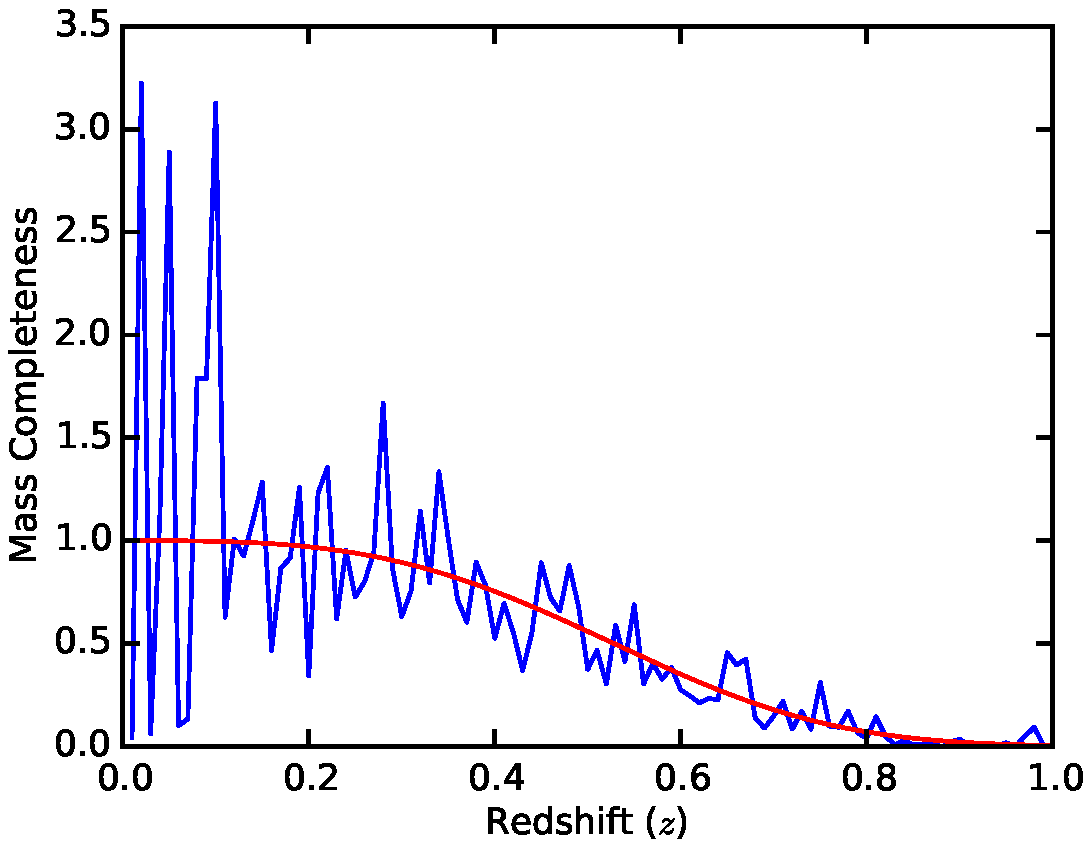
\includegraphics[width=\columnwidth]{mass_completeness.pdf}
\caption{\label{fig:mass_complete} Mass completeness as a function of redshift. The blue line shows the average mass per redshift bin, relative to a smooth universe, across the 23 fields for which we have constructed 3-D mass models. The red line shows the best fit to the data using a functional form of $f(z) = e^{-z^a / b}$ with best fit parameters $a = 3.23$ and $b = 0.183$. We then use this mass completeness function to set the lensing contribution from the smooth background mass density. This allows to self consistently include voids. Because this is a fit to the average across mass models, individual beams can have higher or lower than the mean density of the universe. The only assumption is that the average of our beams should be approximately the mean density of the universe.
}
\end{center}
\end{figure}

In practice, we parameterize the mass completness, $f(z)$, with a simple analytic function. Using all 23 fields for which we have constructed mass models, we fit the average mass per redshift bin, relative to a smooth universe, using a function of the form $f(z) = e^{-z^a / b}$ as shown in Figure \ref{fig:mass_complete}. This function is a generalization of a Gaussian that captures the near-total completeness at low redshift (with $f(z=0) = 1$) and smoothly decreases in a similar manner to our observed mass completeness. We find best fit values of $a = 3.23$ and $b = 0.183$. We adopt this mass completeness function for all subsequent analysis. Because we have used the average across all of our beams instead of fitting each beam individually, this allows for individual beams to be over or under dense compared to the mean density of the universe. The only assumption is that the mean of our total sample is approximately the mean density of the universe. 

\subsection{Generating Mock Lensing Observables} \label{sec:observables}

Next, we place a lens galaxy into our ENV/LOS mass models, put a variety of sources behind it, and solve the lens equation to generate ``mock'' lenses.\footnote{All of our simulations and modeling use the \emph{lensmodel} package \citep{Keeton01}.}  We treat the main lens galaxy using a ellipsoidal power law model given by
\begin{equation}
\label{eqn:powerlaw}
\kappa = \frac{b^{2-\eta}}{2 \xi^{2-\eta}}
\quad\mbox{where}\quad
\xi^2 = x^2 + \frac{y^2}{(1-e)^2}
\end{equation}
Here $\xi$ is the elliptical radius and $e$ is the ellipticity.  The power law index $\eta$ is chosen so the enclosed mass scales as $M(r) \propto r^\eta$.
The Einstein radius for this model is $R_E = b \eta^{\eta - 2}$. Our initial models use $\eta = 1$ which corresponds to a singular isothermal ellipsoid.

We treat the azimuthal angle of the main lens galaxy and the position of the source as nuisance parameters to marginalize.  Specifically, we draw random values for the lens galaxy orientation from a uniform distribution.  We choose source positions from a magnification weighted distribution to approximate the magnification bias that is present in real observations \citep[see][]{Keeton04}. Overall, we generate a sample of 300 quad and 300 double mock image configurations for each mass model.

We use the full recursive lens equation (eq.\ \ref{eqn:full_mp} with no approximations) to ray trace through our mass models and generate mock lensing observerables: image configuration, image positions, time delays, and flux ratios. We imagine observing these lenses with fiducial measurement uncertainties of 3 milliarcseconds for the positions of the lensed images and the main galaxy, $5\%$ for the fluxes, and 1 day for the time delays. These values are typical of observations with instruments such as \emph{HST} and monitoring campaigns such as COSMOGRAIL \citep{Eigenbrod05}. We do not explicitly add scatter to the mock data; preliminary tests indicate that such measurement noise introduces a ``floor'' in the $\chi^2$ values and the scatter in recovered lens parameters but does not qualitatively change our results.

Two-image lens systems have the following observables:
\begin{itemize}
\item $2\times 2$ image  positions ($x,y$)
\item 2 fluxes
\item 1 time delay 
\item $1\times 2$ lens galaxy position ($x,y$)
\end{itemize}
giving a total of 9 constraints.

By contrast, four-image systems have:
\begin{itemize}
\item $4\times 2$ image positions ($x,y$)
\item 4 fluxes
\item 3 time delays
\item $1\times 2$ lens galaxy position ($x,y$) 
\end{itemize}
giving a total of 17 constraints.



%%%%%%%%%%%%%%%%%%%%%%%%%%%%%%%%%%%%%%%%%%%%%%%%%%%%%%%%%%%%%%%%%%
\subsection{Fitting Lens Models \label{sec:lensmodels}}
%%%%%%%%%%%%%%%%%%%%%%%%%%%%%%%%%%%%%%%%%%%%%%%%%%%%%%%%%%%%%%%%%%

We can then fit the simulated observables as we would for real lens systems. We consider three types of models that treat the ENV/LOS in different ways to see if we can recover the true, input lens galaxy parameters and the Hubble constant. We consider the following models:
(1) The ``Lens-Only'' model ignores ENV/LOS effects altogether.
(2) The ``Lens+Shear'' model attempts to account for ENV/LOS effects by fitting an external shear in the main lens plane \citep[e.g.,][]{Suyu13}.
(3) The ``3-D Lens'' model uses our multi-plane framework developed in M14. However, most (or all) of the ENV/LOS galaxies are treated using the tidal approximation. This allows us to disentangle non-linear effects, which are accounted for in our 3-D Lens models, and higher order terms which are not.

The models all have the following 10 free parameters:
\begin{itemize}
\item Source position ($x,y$)
\item Source flux
\item Hubble constant ($h$)
\item Einstein radius of the main lens galaxy
\item Lens galaxy position ($x,y$).
\item Lens galaxy ellipticity and orientation ($e,\theta_e$)
\item Lens galaxy power law index ($\eta$)
\end{itemize}
The Lens+Shear model has two additional free parameters that characterize the external shear; we use the pseudo-Cartesian components of the shear, $\gamma_c = \gamma \cos 2\theta_\gamma$ and $\gamma_s = \gamma \sin 2\theta_\gamma$.

Given the numbers of parameters and constraints, quad lenses are well constrained with 7 degrees of freedom (dof) for the Lens-Only and 3-D Lens models and 5 dof for the Lens+Shear model. Double lenses are, however, underconstrained with $-1$ dof for the Lens-Only and the 3-D Lens models and $-3$ dof for the Lens+Shear model.

Because the Lens+Shear model has a different number of dof, care must be taken when comparing the results to the other models. We scale the $\chi^2$ value by the 95\% confidence limit for the number of dof to ensure a fair comparison across model types.

In some cases it may be reasonable to put priors on the lens galaxy ellipticity and orientation based on the light profile \citep[e.g.,][]{Bolton08}, but in lensing there is not always a strong relation between the light and mass \citep[][and references therein]{Bruderer15}. Therefore we do not place any priors on the lens galaxy parameters.  We do assume a weak Gaussian prior on the Hubble constant, $h = 0.71 \pm 0.3$, which ensures that models are reasonable but otherwise has little effect on the results for quad lenses.  The prior plays a stronger role in double lenses since they are underconstrained.  Overall, the results from double lenses are qualitatively similar to those from quad lenses but considerably broader.  For the remainder of the discussion we focus on quad lenses because they are better constrained.


In all cases, the model parameters are varied to find the best fit and allowed range.  We seek to understand how the assumptions and approximations in the various models cause parameters to shift away from their true values. 
The Lens-Only models ignore the ENV/LOS entirely, so they serve as control test: the best fit values for the lens galaxy parameters and the Hubble constant move away from the truth in an attempt to account for the LOS/ENV effects allowing us to characterize the overall importance of ENV/LOS effects. The Lens+Shear models have two extra free parameters, and we aim to test whether the shear can account for ENV/LOS effects well enough to provide robust constraints on the Hubble constant. Finally, the 3-D Lens models are based on the same mass models that were used to generate the mock lensing observables. The analysis is not circular, however, because the fits treat most or all of the ENV/LOS galaxies using the tidal approximation (whereas the mock data are generated with the full multi-plane lens equation). This approach allows us to isolate the effects of higher order terms beyond the shear and convergence. Also, even with perfect knowlege of the ENV/LOS, there may be degeneracies between model parameters in the 3-D Lens models that we will explore below. 



For the recovered lens quantities, we use Markov Chain Monte Carlo methods to calculate the full posterior probability distribution. When presenting marginalized results for a given lens parameter, we show the median value of the fitted parameters and estimate the scatter by measuring half of the difference between the $16^{th}$ and $84^{th}$ percentiles. When plotting results, we show fractional changes in the fitted parameters to emphasize the variation.

 We now have all of the machinery in place to study the ENV/LOS contribution to lensing. We now turn to the results of our simulations.


%%%%%%%%%%%%%%%%%%%%%%%%%%%%%%%%%%%%%%%%
\section{Results}
%%%%%%%%%%%%%%%%%%%%%%%%%%%%%%%%%%%%%%%%

To understand the contribution of the ENV/LOS to lensing, we break the problem into four pieces. We first examine the perturbations due to individual ENV/LOS galaxies to understand what combination of mass, projected offset, and redshift determine a perturber’s importance  (Section \ref{sec:Individual}). We then apply the lessons to realistic mass models that contain hundreds of ENV/LOS galaxies (Section \ref{sec:Environments}). After that, we fit the mock lensing observables generated with our realistic mass models to determine how well different types of models can recovered the input galaxy parameters and cosmology (Section \ref{sec:fitting}). Finally, we place different lens systems into the ENV/LOS mass models to understand how the mass and ellipticity of the lens galaxy and the position of the source affect a lens's sensitivity to ENV/LOS effects when inferring the Hubble constant (Section \ref{sec:ImageConfigs}). 

%%%%%%%%%%%%%%%%%%%%%%%%%%%%%%%%%%%%%%%%
\subsection{Which Individual Environment/LOS Galaxies are the Most Important?}
\label{sec:Individual}
%%%%%%%%%%%%%%%%%%%%%%%%%%%%%%%%%%%%%%%%
\begin{figure}[t]
\begin{center}
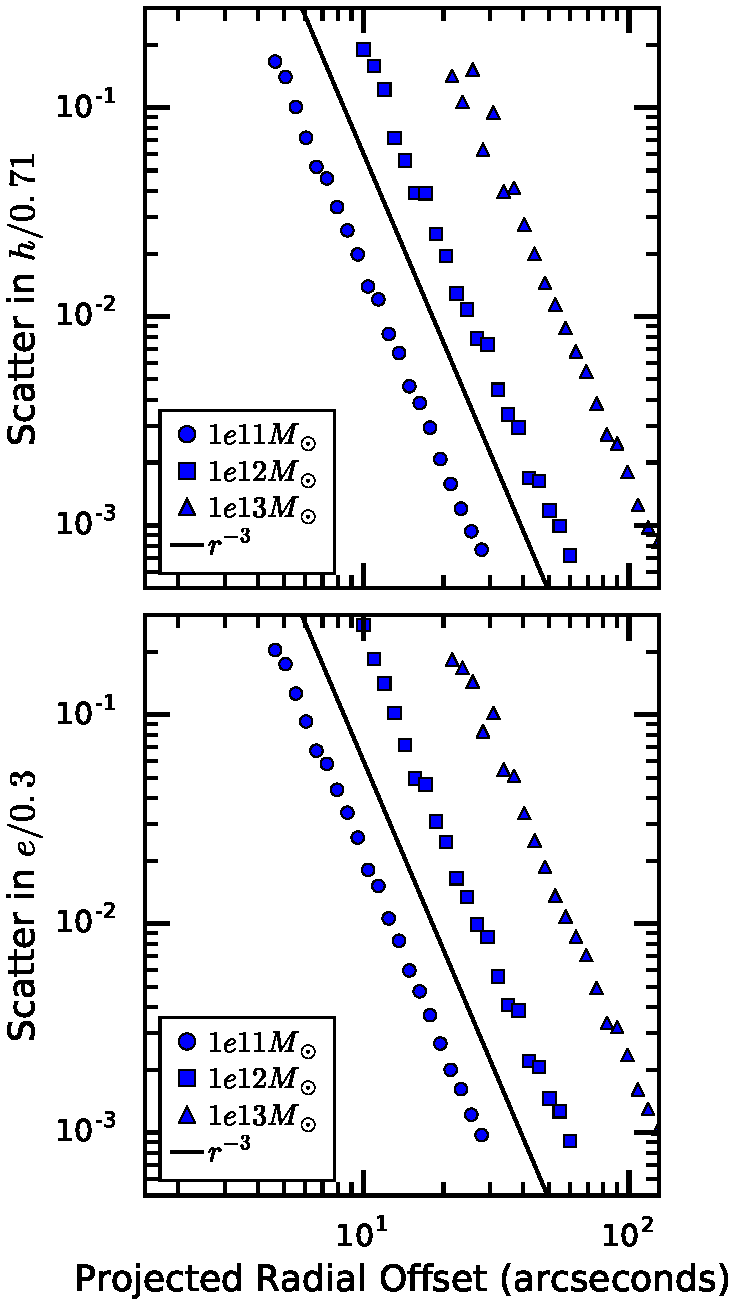
\includegraphics[width=\columnwidth]{toymass_compare.pdf}
\caption{\label{fig:toyr3} Deviations in lens model parameters for simulations with a single perturbing galaxy at the same redshift as the main lens galaxy.  The horizontal axis is the radial offset of the perturber, and the vertical axis is the scatter in recovered values of the Hubble constant ($h$, top) and ellipticity ($e$, bottom). The points show results from simulations for three decades in the perturber's mass. The parameter deviations follow a $r^{-3}$ power law (indicated with a line) because our models omit third-order terms and higher in the lens potential. The deviations also scale with perturber mass as $M \propto R_p^2$. Thus, understanding lens potential perturbations provides a robust way to characterize a perturbing galaxy's effect on the Hubble constant.%
}
\end{center}
\end{figure}

While there hundreds of galaxies in our beams, they are not equally important for lensing.  Conceptually, we want to understand what properties control an individual perturber's influence on the lensed images. When characterizing an individual perturber, we test the effects of mass, projected offset from the main lens galaxy, and redshift. We initially control for redshift, placing the perturbing galaxy at the same redshift as the main lens but varying the mass and projected offset (Section \ref{sec:toylos}). We then move the perturbing galaxy in redshift (Section \ref{sec:frontback}). Based on the results from M14, we expect there to be a difference between perturbers in the foreground and background of the main lens due to non-linear effects that we aim to quantify. We use both equations and simulations to identify a quantity, based on the flexion produced by a perturbing galaxy, that characterizes how much a given galaxy affects the recovered value of the Hubble constant.

\subsubsection{Massive Galaxies Projected Near the Lens are More Important \label{sec:toylos}}

We begin our characterization of individual perturbing galaxies with the simplest case: we examine one main lens galaxy and one perturbing galaxy in the same plane (removing any redshift effects). We first derive analytic expectations for how an individual perturbing galaxy affects the lens potential, and then show that the deviations in the recovered Hubble constant scale in the same way as the lens potential perturbations.

Consider a single main lens galaxy with deflection, $\al_{g}$, and a single perturbing galaxy with deflection, $\al_p$. Both are at the same redshift in this case. It is useful to define the lensing potential as
\begin{equation}
\al \equiv \nabla \phi.
\end{equation}
If the perturbing galaxy does not overlap the lensed images, its gravity is the same as a point mass so we can write the lens potential as
\begin{equation}
\phi_p = R_p^2 \ln \left| \x - \vec{r} \right| 
\end{equation}
where $R_p$ is the Einstein radius of the perturber, $\x$ is the image position in the redshift plane of the perturber, and $\vec{r}$ is the position of the perturber. If we let $|\x| = x$, $|\vec{r}| = r$, and $\theta=$ the angle between the perturber and the image position as measured from the origin, we can rewrite the potential using the law of cosines as
\begin{equation}
\phi_p = \frac{1}{2}R_p^2 \ln(r^2 + x^2 - r x \cos\theta).
\end{equation}
If the perturbing galaxy is far from the lensed images, then $x \ll r$ and we can expand the potential in a Taylor series:
\begin{eqnarray}
\phi_p &=& R_p^2 \left[ \ln(r) - \cos(\theta) \frac{x}{r}  - \frac{1}{2} \cos(2\theta) \frac{x^2}{r^2} \right. \nonumber\\
&& \qquad\left. - \frac{1}{3}\cos(3\theta)\frac{x^3}{r^3}  + \ldots\right].
\end{eqnarray}
This expression can be extended beyond a point mass model as
\begin{equation}
\phi_p = \phi(0) + \alpha^i(0) x^i + \frac{1}{2}\Gamma^{ij} x^i x^j+ \frac{1}{6} \sF^{ijk} x^i x^j x^k + \ldots 
\end{equation}
where we have adopted the Einstein convention of summing over repeated indices and defined the tidal and flexion\footnote{Throughout this work, we refer to  third-order terms collectively as ``flexion'' terms, but see \citet{Bacon06} for more discussion.} tensors:
\begin{eqnarray}
\Gamma^{ij} &\equiv& \left. \frac{\partial^2 \phi_p}{\partial x^i \partial x^j} \right|_{x=0} , \\
\sF^{ijk} &\equiv&  \left. \frac{\partial^3 \phi_p}{\partial x^i \partial x^j \partial x^k} \right|_{x=0} .
\end{eqnarray}
For a point mass, the tidal and flexion amplitudes scale as $\Gamma \propto R_p^2/r^2$ and $\sF \propto R_p^2/r^3$.

\begin{figure}[t]
\begin{center}
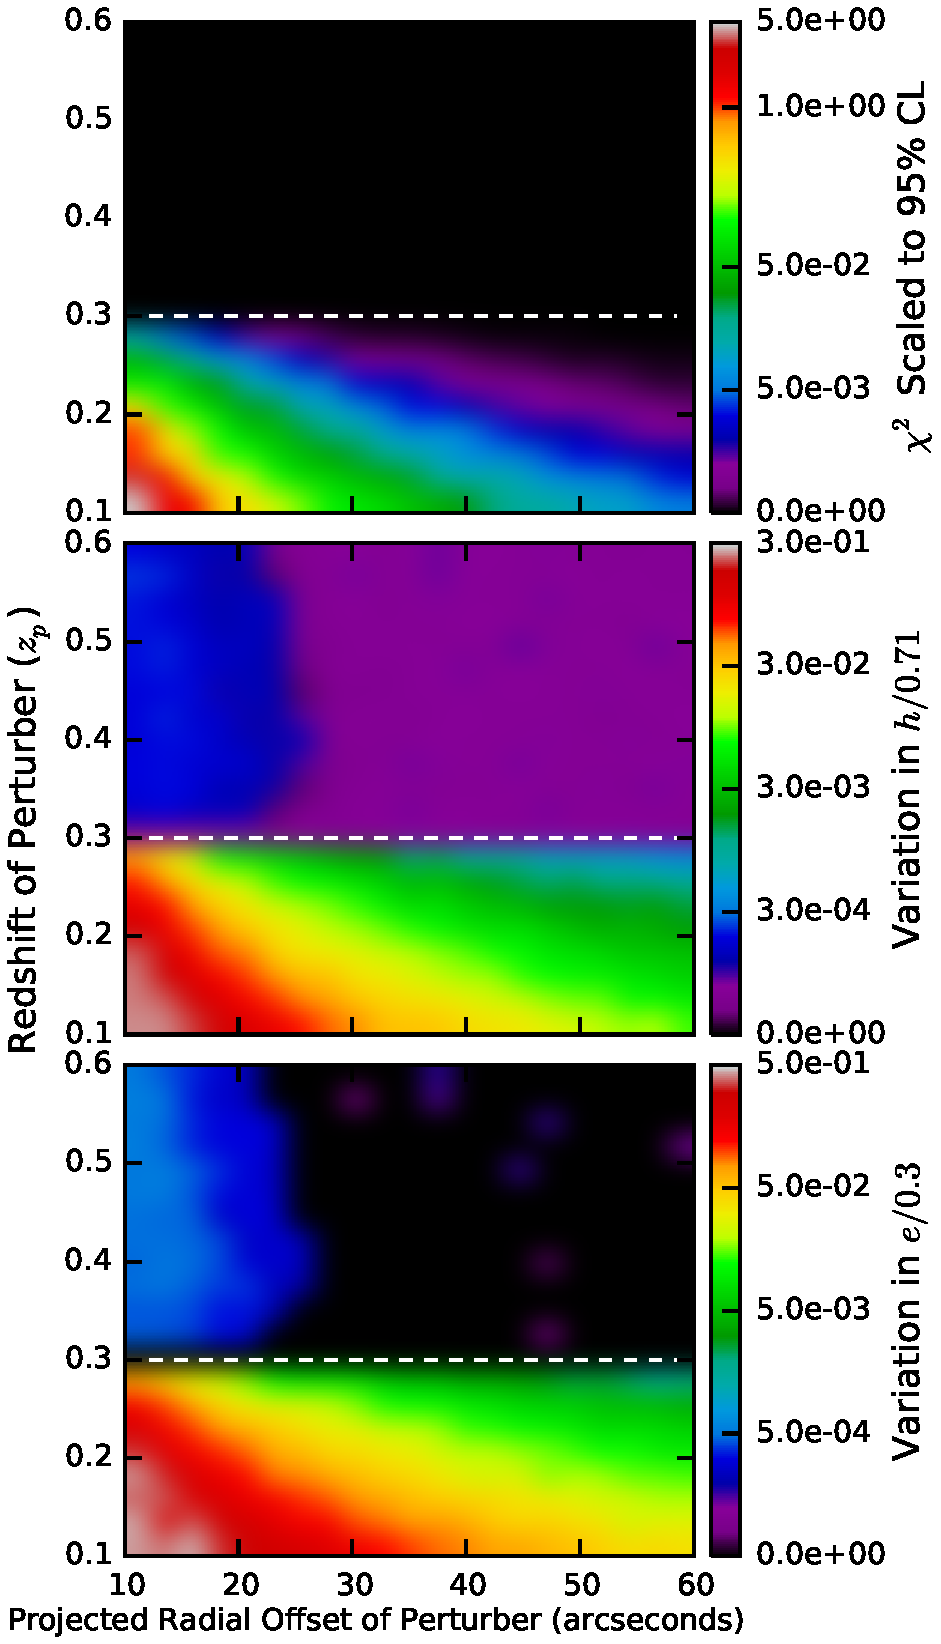
\includegraphics[width=1.0\columnwidth]{frontback.pdf}
\caption{\label{fig:frontback} Recovered lens model parameters for simulations with only tidal effects from an LOS perturber. The simulations shown here do not include higher order terms, to emphasize non-linear effects.  The main lens has a redshift of $z_{\rm{lens}} = 0.3$ (marked by the white dashed line) and the perturber has a mass of $10^{12}\, M_\odot$.  We use an $\asinh$ color scaling for dynamic range; (at large values, $\asinh$ acts like a logarithm, but at small values, it becomes linear).  When the perturber is in the background, an effective shear can account for the LOS effects (see eq.\ \ref{eqn:Geff}).  When the perturber is in the foreground, however, there are non-linear effects that cannot be mimicked by a shear in the lens plane.
}
\end{center}
\end{figure}

In the expansions, the zeroth order terms correspond to shifts in the zeropoint of the potential, which are unobservable.  The first order terms correspond to a uniform deflection, which can be absorbed by translating the source plane.  Therefore only the terms at second order and higher have observable consequences.

To quantify the environmental effects, we run simulations with an SIE main lens galaxy and a point mass perturber.  We choose the Einstein radius of the main lens to be $R_E = 1.0''$, and we place the lens and perturber at redshift $z_{\rm{lens}} = z_p = 0.3$ in front of a source at redshift $z_{\rm{src}} = 2.0$.  We consider three decades of perturber mass.  Figure \ref{fig:toyr3} shows the results in terms of scatter in the recovered values of the Hubble constant $h$ and the ellipticity $e$.

The parameter scatter increases as the perturber gets closer to the main galaxy and higher order terms become more important.  The scalings follow power laws that are consistent with the deviations in the lens potential. Our models omit third-order terms and higher, so we expect the scatter to scale as $r^{-3}$. The scatter in the ellipticity and the Hubble are both proportional to the mass of the perturbing galaxy. 

Therefore, the scatter in the recovered Hubble constant created by an individual perturbing galaxy is proportional to $M / r^3$ (note that $ M \propto R_p^2$ for a point mass), which is the same scaling as the deviations in the lens potential. These results quantify our intuition that massive galaxies near the main lens are important for lensing. 

Below, we will use these mass and offset scalings to characterize the strength of a perturbing ENV/LOS galaxy, but this current analysis only applies if the perturbing galaxy is at the same redshift as the main lens.

\subsubsection{Foreground Pertubers are More Important than Background}
\label{sec:frontback}

Now that we understand the mass and offset scalings, we examine how the redshift of the perturbing galaxy affects its contribution to the lens potential. 

For a single perturbing galaxy, the lens equation \ref{eqn:full_mp} has the form
\begin{equation}
\x_2 = \x_1 - \beta_{1\,2} \al_1(\x_1)
\end{equation}
and
\begin{equation}
\x_s = \x_1 - \beta_{1\,s} \al_1(\x_1) - \beta_{2\,s} \al_2(\x_2).
\end{equation}
Combining these equations, recalling that $\beta_{i\,s} \equiv 1$, and setting $\beta \equiv \beta_{1\,2}$ lets us write the two-plane lens equation as
\begin{equation}
\x_s = \x_1 - \al_1(\x_1) - \al_2\left(\x_1 - \beta \al_1(\x_1)\right).
\label{eqn:twoplane}
\end{equation}
In the following discussion it is useful to recall that $\beta$ varies monotonically with redshift, ranging from $\beta = 0$ when $z_p = z_{\rm{lens}}$ to $\beta = 1$ when the perturber redshift reaches either $z_p = 0$ (for a foreground perturber) or $z_p = z_{\rm{src}}$ (for a background perturber).

To make further progress, we need to distinguish situations when the perturber is in front of or behind the main lens galaxy. In M14, we showed that background perturbers produce an additional shear while foreground perturbers produce non-linear effects.

\begin{figure}[t]
\begin{center}
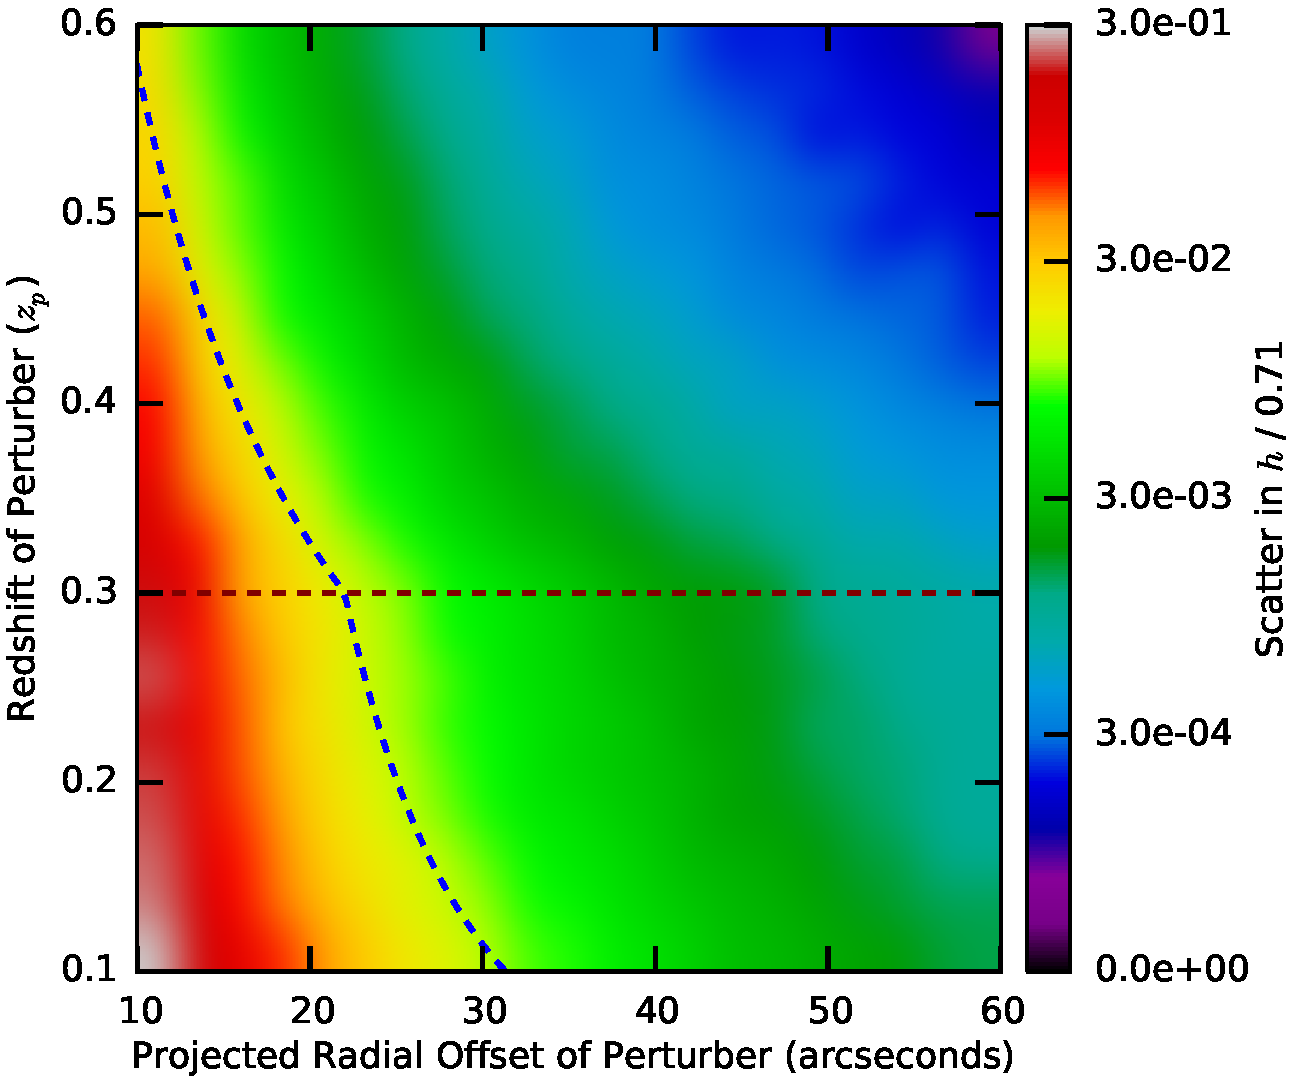
\includegraphics[width=\columnwidth]{toyh.pdf}
\caption{\label{fig:toyhd3x} Scatter in the Hubble constant, $h$, recovered from 3-D Lens models for perturbers at different projected offsets and redshifts.  The main lens has a redshift of $z_{\rm{lens}} = 0.3$ which is marked with a dotted line, and the perturbing galaxy has a mass of $10^{12}\,M_\odot$.  The dashed line shows a contour of constant flexion shift, $\Delta_3 x$, from equations \ref{eqn:backgroundd3x} and \ref{eqn:foregroundd3x} (picking a different value of $\Delta_3 x$ would simply rescale the contour). The effects due to a perturber in the background are downweighted (see equation \ref{eqn:backgroundd3x}), and therefore the perturber needs to be closer in projection to have the same effect than as if it were at the same redshift as the lens. In the foreground, the curve flares out, implying that foreground perturbers can be farther away in projection to have the same effect if they were at the lens redshift. This occurs because the Einstein radius of a point mass increases as redshift decreases, yielding stronger lensing effects. The curve matches the shape of the color contours, indicating that our theoretical expression from the lens potential captures the redshift dependence of LOS effects in the recovered parameters, like the Hubble constant.  Thus, we can use the flexion shift to compare effects of LOS galaxies even if they are at different redshifts.
}
\end{center}
\end{figure}

\medskip
\centerline{\emph{Lens Potential Perturbations}}
\centerline{\emph{from a Background Galaxy}}
\medskip

Suppose the perturbing galaxy is in the background. The first part of this discussion parallels \citet{Keeton03}.  We have $\al_1 = \al_g$ and $\al_2 = \al_p$. Substituting this into equation \ref{eqn:twoplane} yields
\begin{equation}
\x_s = \x_1 - \al_g(\x_1) - \al_p(\x_1 - \beta \al_g(\x_1)). 
\end{equation}
We Taylor expand $\al_p$ and omit the unobservable terms corresponding to the constant potential and deflection:
\begin{eqnarray}
x^i_s &=& x^i_1 - \alpha^i_g(\x_1) - \Gamma^{ij} (x^j_1 - \beta \alpha^j_g(\x_1)) \\
&&- \frac{1}{2} \sF^{ijk} (x^j_1 - \beta \alpha^j_g(\x_1)) (x^k_1 - \beta \alpha^k_g(\x_1)) + \mathcal{O}(\x_1^4) . \nonumber
\end{eqnarray}
Here we use index notation for clarity.

If we truncate the expansion at tidal terms and return to vector/tensor notation, we can write
\begin{equation}
\label{eqn:background}
\x_s = (\I - \GammaMat) \x_1  - (\I - \beta \GammaMat)\al_g(\x_1) + \mathcal{O}(\x_1^3).
\end{equation}
This equation looks very similar to the single plane lens equation, but with some multiplicative factors. In fact, if we multiply both sides by $(\I - \beta \GammaMat)^{-1}$ from the left, introduce a scaled source coordinate $\vec{u}_{\rm eff} \equiv (\I - \beta \GammaMat)^{-1} \x_s$, and define an effective shear by
\begin{equation}\label{eqn:Geff}
\I -\GammaMat_{\rm eff} \equiv (\I - \beta\GammaMat)^{-1} (\I - \GammaMat) ,
\end{equation}
then we can rewrite equation \ref{eqn:background} as
\begin{equation}
\vec{u}_{\rm eff} = (\I - \GammaMat_{\rm eff}) \x_1 - \al_g(\x_1),
\end{equation}
which is equivalent to the single plane lens equation with an external shear in the lens plane \citep[see also][]{Schneider97}. We are allowed to rescale the source plane because the position of the source is unobservable and we typically only measure the ratio of the fluxes of different images, which is insensitive to the absolute intrinsic luminosity of the source.\footnote{The freedom to rescale the source plane vanishes if the intrinsic luminosity of the source is known.  Thus, lensed standard candles, such as type Ia supernovae \citep{Kelly15, Patel14, Kolatt98}, offer a novel way to break the mass sheet degeneracy.}

In the tidal approximation, we again expect errors in the recovered lens parameters to be associated with the largest terms in the lens potential that have been neglected: the third order flexion terms.  We therefore use the terms involving $\sF$ to quantify the lens potential perturbations.\footnote{Recall from Section \ref{sec:toylos} that the flexion terms scale with mass and projected offset as $M / r^3$; now we generalize now to include redshift.}  We approximate the main lens galaxy as a singular isothermal sphere (SIS) with deflection
\begin{equation}
\al_g = R_E \rhat.
\end{equation}
Then we can write the lens equation \ref{eqn:background} in the tidal approximation as
\begin{equation}
\label{eqn:backgroundorder2}
\x_s = \x_1 - R_E \rhat -  \GammaMat (\x_1 - \beta R_E \rhat).
\end{equation}
For comparison, the lens equation with flexion terms is
\begin{multline}
\x_s = \x'_1 - R_E\rhat -  \GammaMat(\x'_1 - \beta R_E\rhat) \\
- \frac{1}{2}(\x'_1 - \beta R_E\rhat) \sF (\x'_1 - \beta R_E \rhat).
\label{eqn:backgroundorder3}
\end{multline}
where we recognize that the solutions $\x'_1$ of this equation may differ from the solutions $\x_1$ of equation \ref{eqn:backgroundorder2} because of the flexion effects.  If we assume that $\GammaMat \ll 1$ (which applies if this is truly a perturbing galaxy and not a main lens galaxy), and we subtract equations \ref{eqn:backgroundorder3} and \ref{eqn:backgroundorder2}, we can define the image shift caused by third order terms to be $\Delta_3 \x \equiv \x'_1 - \x_1$, and thus find
\begin{equation}
\Delta_3 \x = \frac{1}{2} (\x'_1 - \beta R_E \rhat) \sF (\x'_1 - \beta R_E \rhat).
\end{equation}
Now, if we define the perturber to be colinear with the image position ($\theta  = 0$)\footnote{If we consider all possible angles, the root mean square value has an extra factor of $\sqrt{2}$ that does not affect the scalings.} and assume that the positions of the multiple images are $|\x'_1| \approx |\x_1| \approx R_E$, we can write the magnitude of the flexion shift as
\begin{equation}
\Delta_3 x = \frac{R_E^2 R_p^2}{r^3} (1 - \beta)^2. 
\label{eqn:backgroundd3x}
\end{equation}
We call this quantity, $\Delta_3 x$, the ``flexion shift'' because it characterizes the perturbations to image positions caused by flexion from a perturber. This quantity has units of arcseconds and it gives us a way to quantify and compare the ENV/LOS contributions from different perturing galaxies.

We note that in this derivation, we have used the expression for $\sF$ for a point mass, which is reasonable when the perturber is projected far from the images.  Strictly speaking, $r$ here is the unlensed distance in the redshift plane of the perturber. To convert to offset as observed on the sky $r'$, we use the lens equation to yield $r' = r - \beta R_E$. As long as the perturbing galaxy is many Einstein radii away from the lens, we can put $r' \approx r$.  (If that were not the case, the perturber would need to be treated as a main plane.)

\medskip
\centerline{\emph{Lens Potential Perturbations}}
\centerline{\emph{from a Foreground Galaxy}}
\medskip



We now turn our attention to a perturber in the foreground of the lens. In this case $\al_1 = \al_p$ and $\al_2 = \al_g$, so the lens equation has the form
\begin{equation}
\x_s =\x_1 - \al_p(\x_1) - \al_g(\x_1 - \beta \al_p(\x_1)).
\end{equation}
Taylor expanding $\al_p$ yields
\begin{eqnarray}
x^i_s &=& x^i_1  - \alpha_p^i(0) - \Gamma^{ij}x^j_1 - \frac{1}{2} \sF^{ijk} x^j_1 x^k_1 +\ldots \\
&& - \alpha^i_g \left(x^i_1 - \beta\alpha_p^i(0) - \beta \Gamma^{ij} x^j_1 - \frac{1}{2} \sF^{ijk} x^j_1 x^k_1 + \ldots \right). \nonumber
\end{eqnarray}
Now truncating at tidal terms yields
\begin{equation}
\x_s = (\I - \GammaMat) \x_1 - \al_g\left((\I - \beta\GammaMat) \x_1 + \mathcal{O}(\x_1^3)\right) + \mathcal{O}(\x_1^3).
\end{equation}
This looks similar to equation \ref{eqn:background}, but there is a key difference: instead of just having a multiplicative effect on the source position like the background perturber, the deflection from the foreground perturber enters the lens equation \emph{inside the argument} of the deflection of the main galaxy. A foreground perturber has complicated effects because it creates a difference between the coordinates we see on the sky and the coordinates in the plane of the main lens galaxy. There is no way to define an effective shear that fully captures the non-linear effects of a foreground perturber (see also M14).

In principle, one can define a scaled coordinate based on the argument of the deflection to transform this equation to look like the standard lens equation \citep[e.g.,][]{Schneider97,Keeton03}. This requires care, however, because the new quantities do not correspond to the \emph{observed} image positions that are typically used in lens modeling. An alternative is to rescale the mass of the main lens galaxy to account for the change in the argument of the deflection \citep{Schneider97}, but this also requires care because the mass predicted by the lens models is no longer the true physical mass of the lens. 

To examine the differences between the foreground and background pertubers, we simulated a $10^{12} M_\odot$ perturbing galaxy at a variety of projected offsets and redshifts. To emphasize the contribution from non-linear effects, in this set of simulations we generate the mock data using the tidal approximation (i.e., there are no higher order terms). This allows us to focus entirely on non-linear effects.  Figure \ref{fig:frontback} shows that an external shear can account for a background perturber (to within numerical precision), as discussed above.  By contrast, shear \emph{cannot} mimic the non-linear effects of a foreground LOS galaxy.  

We now seek an expression for the flexion shift $\Delta_3 x$ caused by a foreground perturber to compare to the background case.  Following an analysis similar to that above, and again using an SIS main lens and a point mass perturber, we can write the lens equation in the tidal approximation as
\begin{equation}
\x_s = \x_1 - R_E \rhat - \GammaMat(\x_1 - \beta R_E \rhat) 
\end{equation}
while the lens equation with flexion terms is
\begin{equation}
\x_s = \x'_1 - R_E \rhat - \GammaMat(\x_1 - \beta R_E \rhat) - \frac{1}{2} \x_1 \sF \x_1.
\end{equation}
Subtracting these equations and rearranging yields
\begin{equation}
\Delta_3 \x = \frac{1}{2} \x_1 \sF \x_1.
\end{equation}
In this case, the multiple images form at $\x_2 \approx R_E \rhat$, implying that $R_E \approx \x_1 - \beta \GammaMat \x_1$. If we assume that $\GammaMat \ll 1$ (as above), we can write $\x_1 \approx R_E \rhat$, giving
\begin{equation}
\Delta_3 x = \frac{R_E^2 R_p^2}{r^3}.
\label{eqn:foregroundd3x}
\end{equation}
This equation is similar to equation \ref{eqn:backgroundd3x}, but without any $\beta$ factors. Therefore, not only can foreground perturbers not be mimicked by an external shear because of non-linear effects, but also the effects of background perturbers are downweighted compared to foreground perturbers.

\medskip
\centerline{\emph{Scatter in Lens Model Parameters}}
\centerline{\emph{Tracks Lens Potential Perturbations}}
\medskip

We now use simulations to test whether our expression for the deviation in the lens potential, the flexion shift $\Delta_3 x$ (eqs.\ \ref{eqn:backgroundd3x} and \ref{eqn:foregroundd3x}), provides a useful way to characterize the importance of ENV/LOS perturbers and their contribution to the recovered lens parameters and Hubble constant. For these simulations, we fix the perturber mass to be $10^{12}\,M_\odot$ but vary its projected offset and redshift. In these simulations, we treat the perturber as a point mass, which is not a valid assumption when the projected offset or redshift is small, but is reasonable in the regime where we anticipate using the tidal approximation.  Figure \ref{fig:toyhd3x} shows the scatter in the recovered value of the Hubble constant (the median value is not shown because it matches the input value; there is no bias).  Generally speaking, the scatter increases as the offset decreases and higher order terms become more significant. In the background, the perturber's effects become weaker as the redshift offset increases because of the $\beta$ factors in equation \ref{eqn:backgroundd3x}; while in the foreground, the perturber's effects become stronger as $z \to 0$ because its angular Einstein radius increases.  Both of these scalings are well described by our functional form for $\Delta_3 x$, which indicates that we have successfully defined a quantitiy to characterize the contribution of perturbing galaxies. 

Many lens systems have significant contributions from in their local environment, (e.g., HE0435$-$1223 has a neighbor, \citealt{Kochanek06}; while MG0414+0534 \citep{Tonry99}, RXJ1131$-$1231 \citep[hereafter RXJ1131][]{Sluse03}, and B2114+022 \citep{King99} all have satellites that are presumably close enough to matter), and while some models do treat nearby perturbers exactly \citep[e.g.,][]{Kochanek06, Fadely12}, typically the decision whether to include a neighbor galaxy in a model is \textit{ad hoc}. The flexion shift, $\Delta_3 x$, provides a quanitative criterion to compare the importance of LOS galaxies even if they are at different redshifts. Any given perturber can be treated with the tidal approximation if its $\Delta_3 x$ value is small, but it must be treated explicitly if its $\Delta_3 x$ value is large.

\subsection{Characterizing Realistic Beams\label{sec:Environments}}

\begin{figure*}[t]
\begin{center}
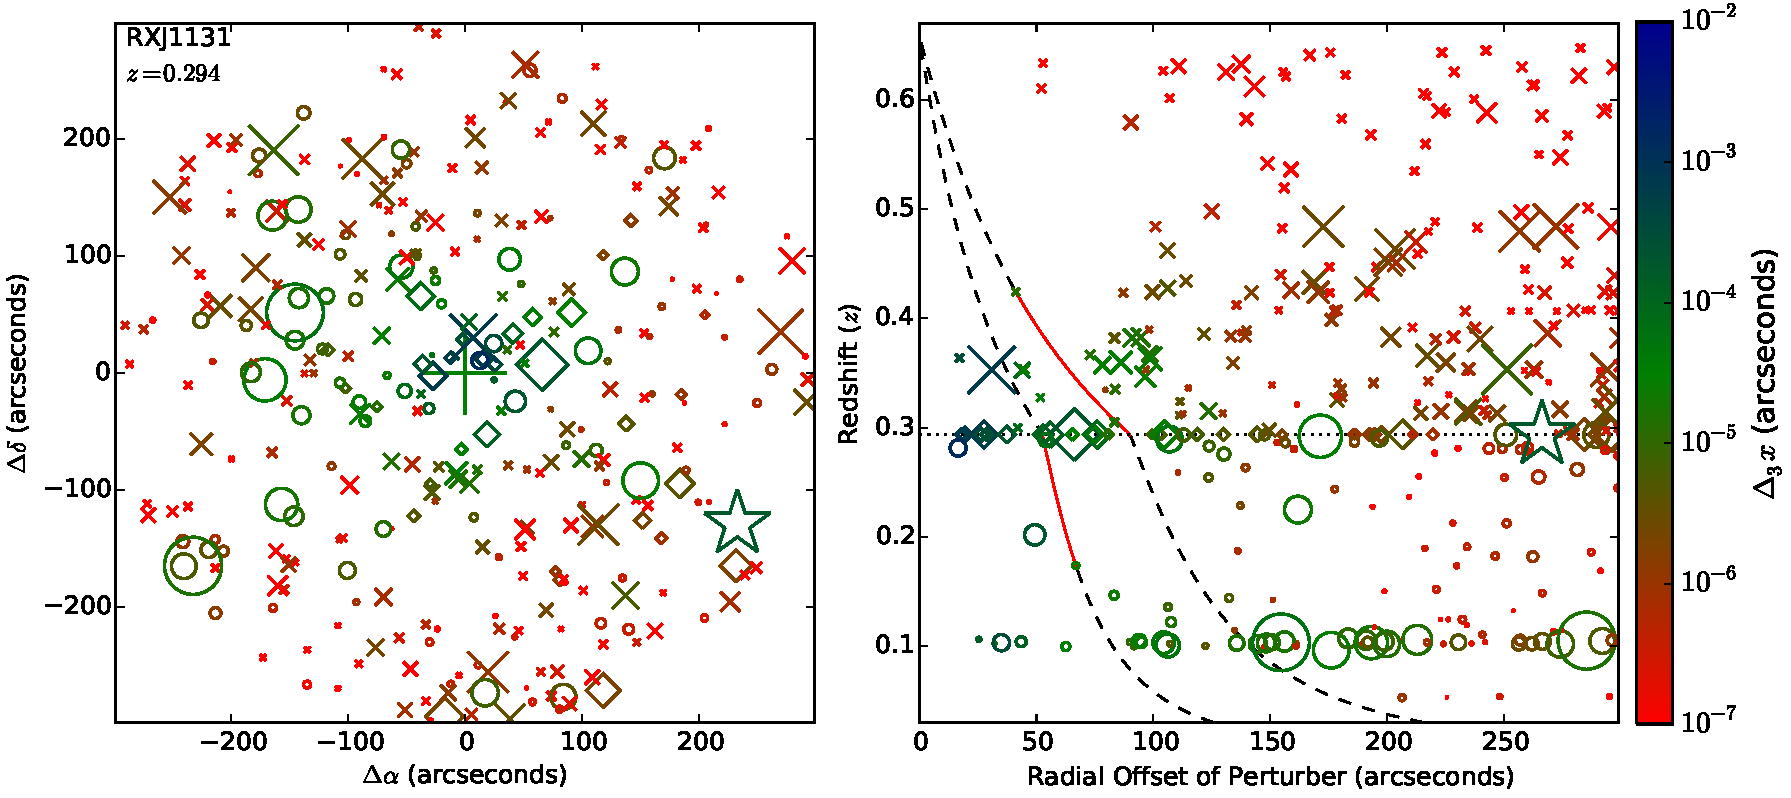
\includegraphics[width=1\textwidth]{RXJ1131_fieldrz.pdf}
\caption{\label{fig:fieldrz} Illustration of the flexion shift for galaxies in the field of RXJ1131.  In the left panel, each galaxy is shown at its position on the sky.  The area of each point is proportional to the mass of the galaxy.  X's and O's mark galaxies behind and in front of the main lens galaxy, respectively, while diamonds mark members in the group around the main lens, and the star indicates the location of the common group halo.  The color of the points represents the strength of the lensing effects measured by the flexion shift $\Delta_3 x$. The right panel shows the same galaxies plotted in the $r$-$z$ projection, similar to Figures \ref{fig:frontback} and \ref{fig:toyhd3x}. The main lens redshift is indicated by the dotted line. Two $\Delta_3 x$ contours have been shown to guide the eye. The red section of the contour illustrates how to map a perturbing galaxy to its effective offset as if it were in the main lens plane. There is no simple radial cut that selects the most important LOS galaxies; a more complicated quantity like the flexion shift, $\Delta_3 x$, is necessary.%
}
\end{center}
\end{figure*}


\begin{figure}[!h]
\begin{center}
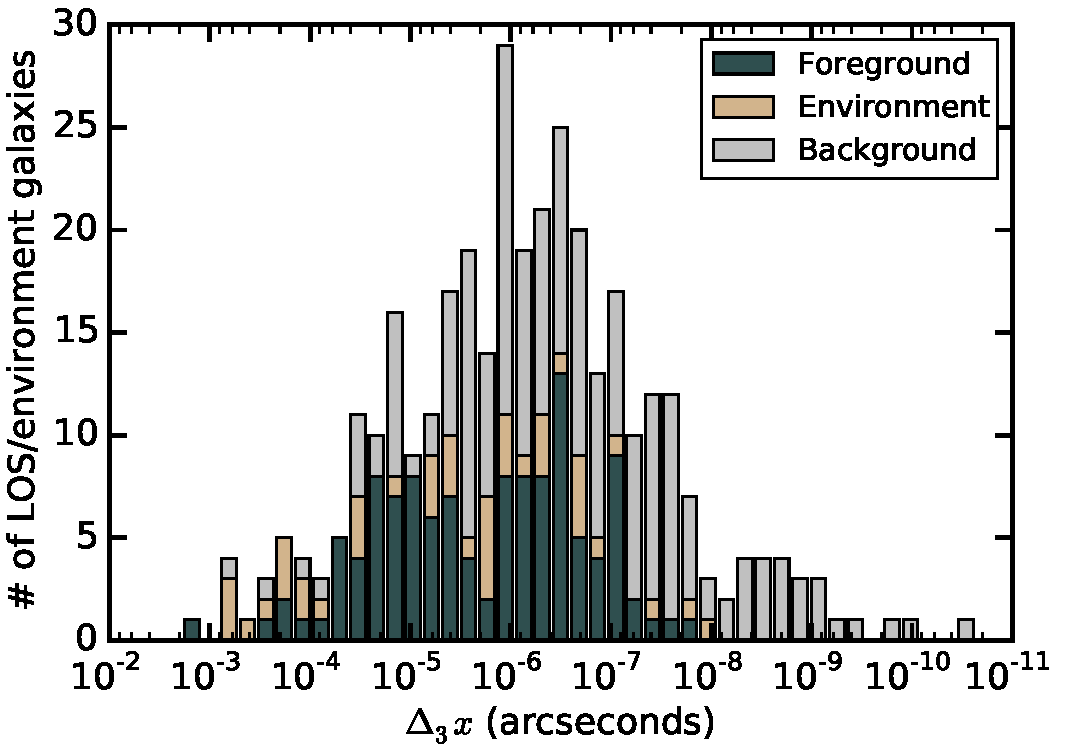
\includegraphics[width=1\columnwidth]{RXJ1131_dx3_hist.pdf}
\caption{\label{fig:d3xhist} Histogram of flexion shifts for galaxies within 5' of RXJ1131.  The dark (light) gray bins represent perturbing galaxies in the foreground (background) of the main lens galaxy, while the silver bins in between correspond to group members in the immediate environment of the main lens. The range of flexion shifts for this field spans $\sim 8$ orders of magnitude. For reference, when generating our $\chi^2$ values, we have assumed a positional uncertainty of $3 \times 10^{-3}$ arcseconds. Few individual perturbing galaxies have that large of flexion shift, but the cumulative flexion is easily larger than our assumed measurement uncertainties. As anticipated, foreground perturbers and group members tend to have larger $\Delta_3 x$ values than background perturbers.%
}
\end{center}
\end{figure}


\begin{figure*}
\begin{center}
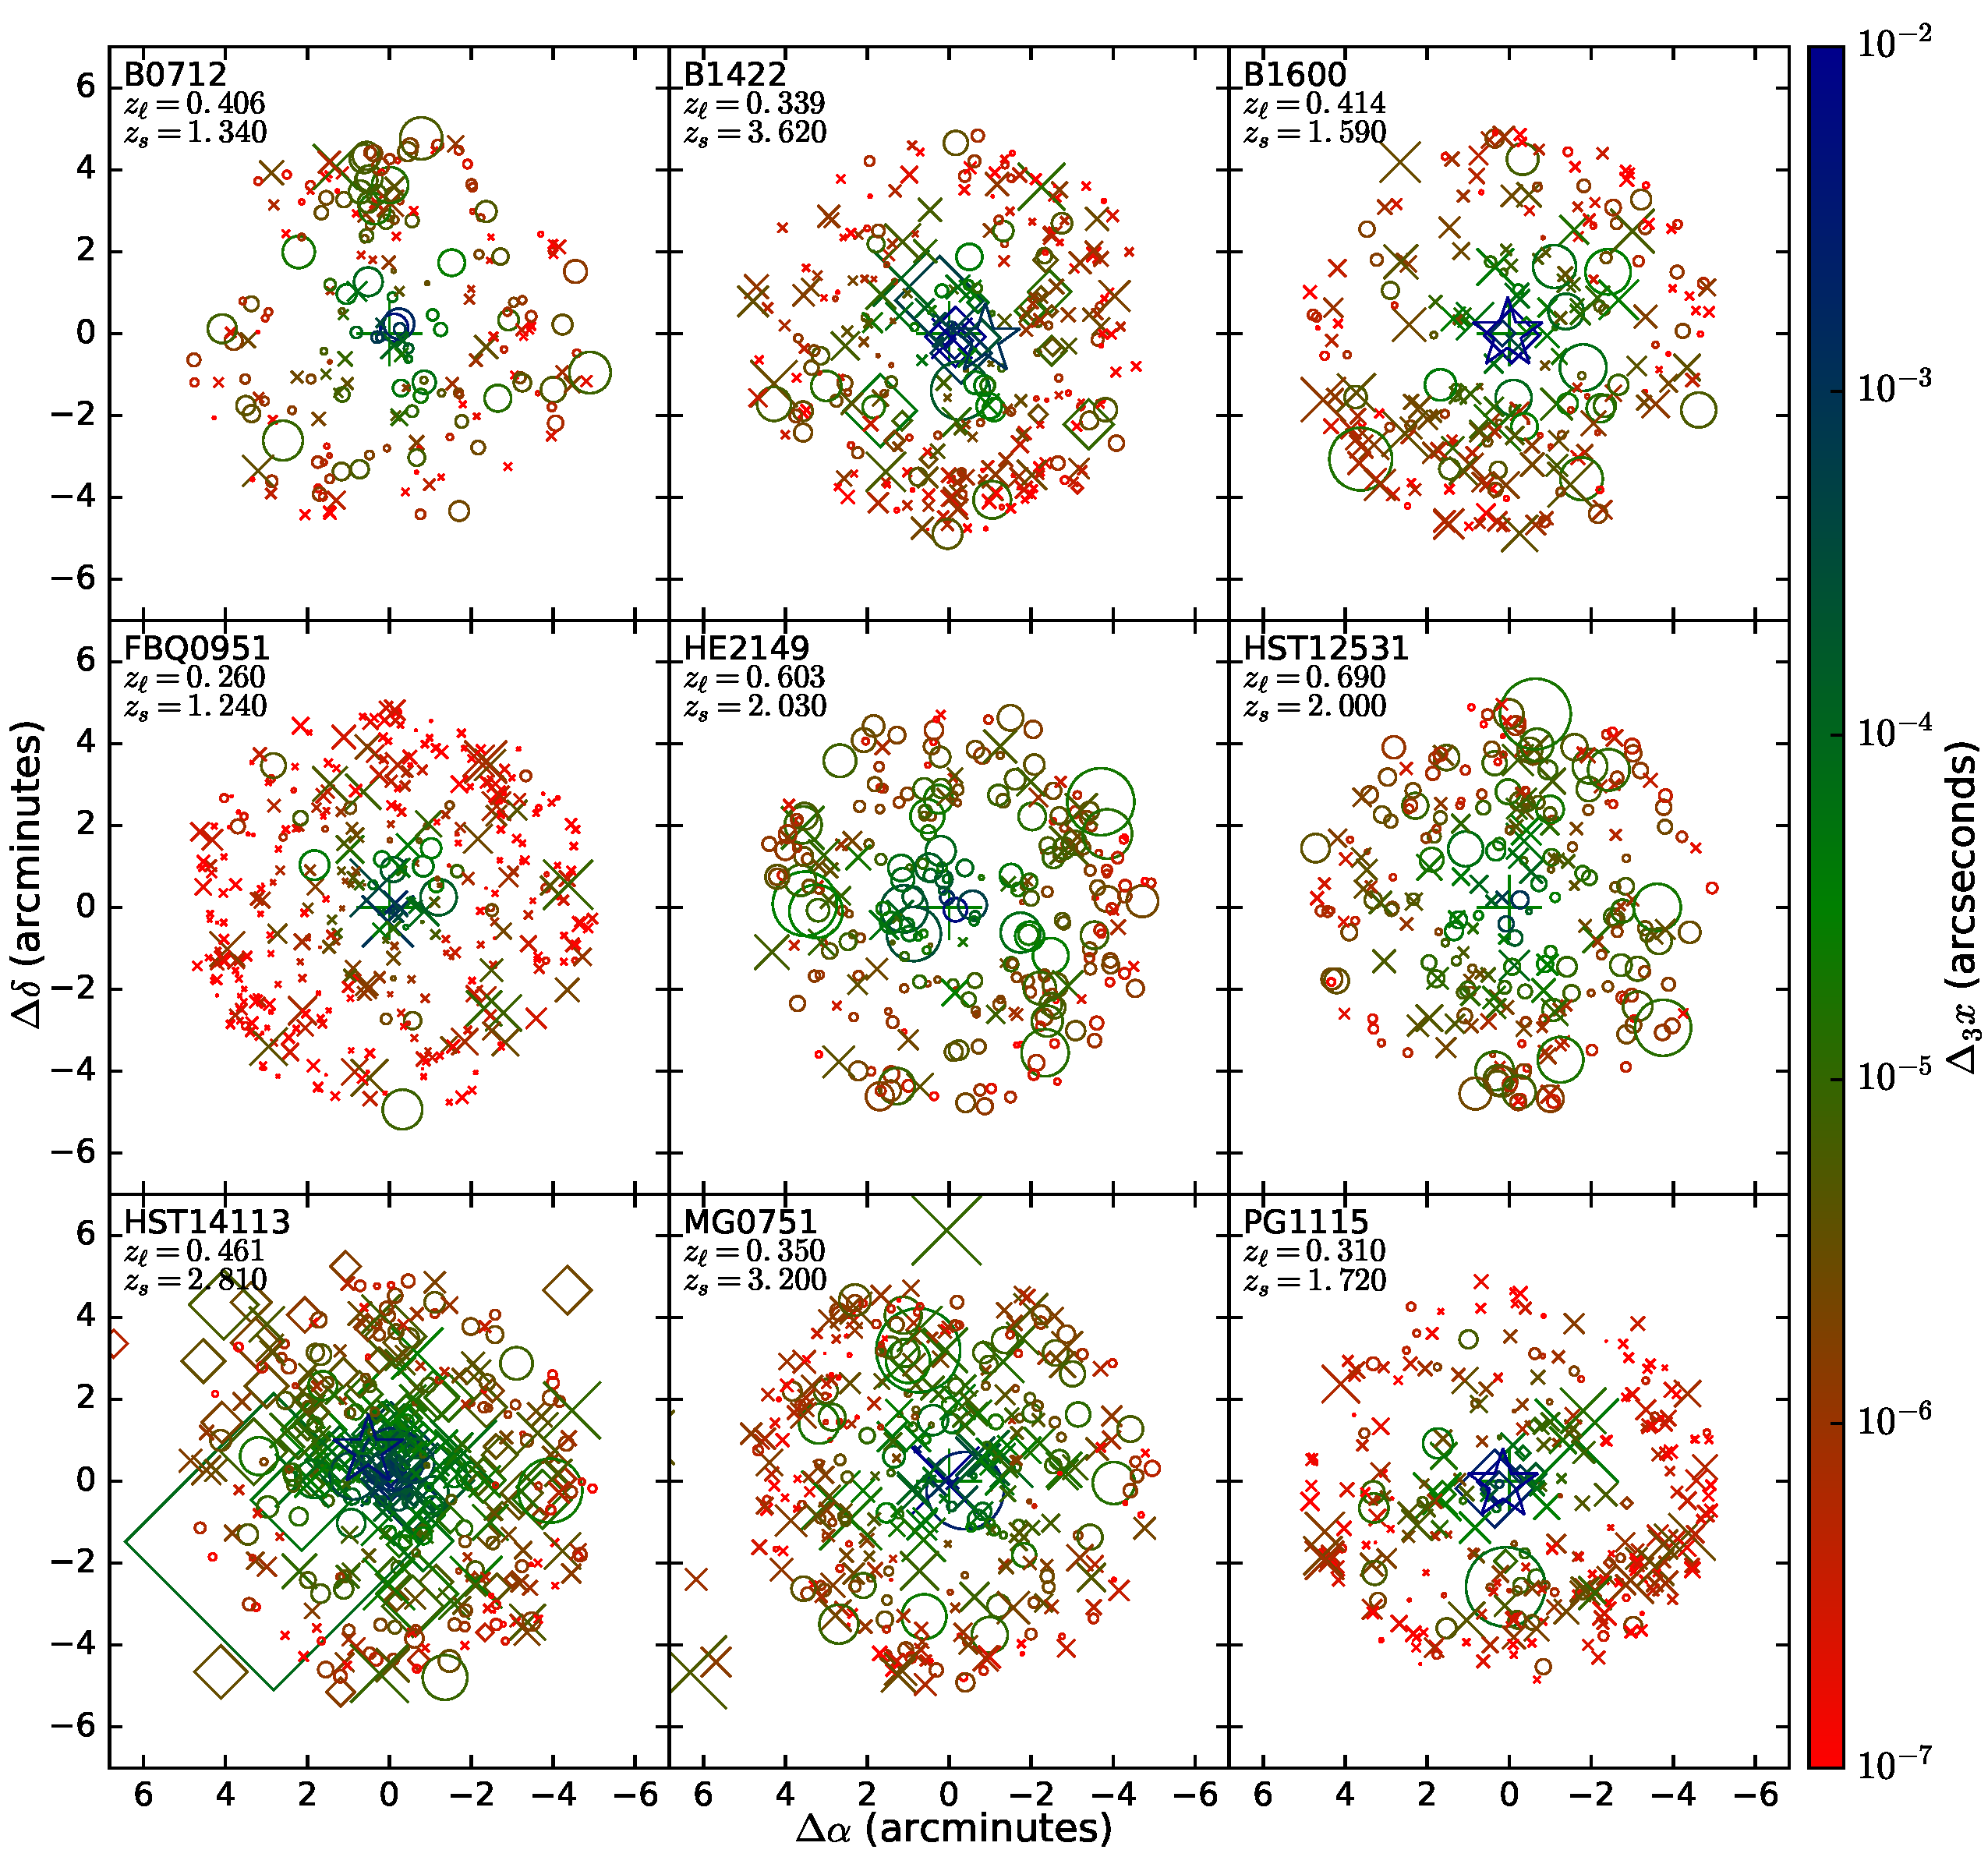
\includegraphics[width=1\textwidth]{allfields.pdf}
\caption{\label{fig:allfields} Illustration of the flexion shifts, $\Delta_3 x$, for perturbing galaxies in nine lens fields (similar to the left panel in Fig.\ \ref{fig:fieldrz}). Each galaxy in the mass model is shown in projection on the sky. The area of each point is proportional to the mass of the galaxy. X's are behind the main lens galaxy, while O's are in the foreground. Diamonds represent group members, while stars indicate the locations of group halos. The color of the points represents the strength of the higher order terms characterized by the flexion shift, $\Delta_3 x$. There is dramatic variation in the ENV/LOS strengths across the different fields, implying that each field needs to be treated on an individual basis. For all of the fields shown here, there is no simple radial cut that would capture all of the important galaxies: a more complicated quantity like the flexion shift is necessary. 
}
\end{center}
\end{figure*}

\begin{figure}[t]
\begin{center}
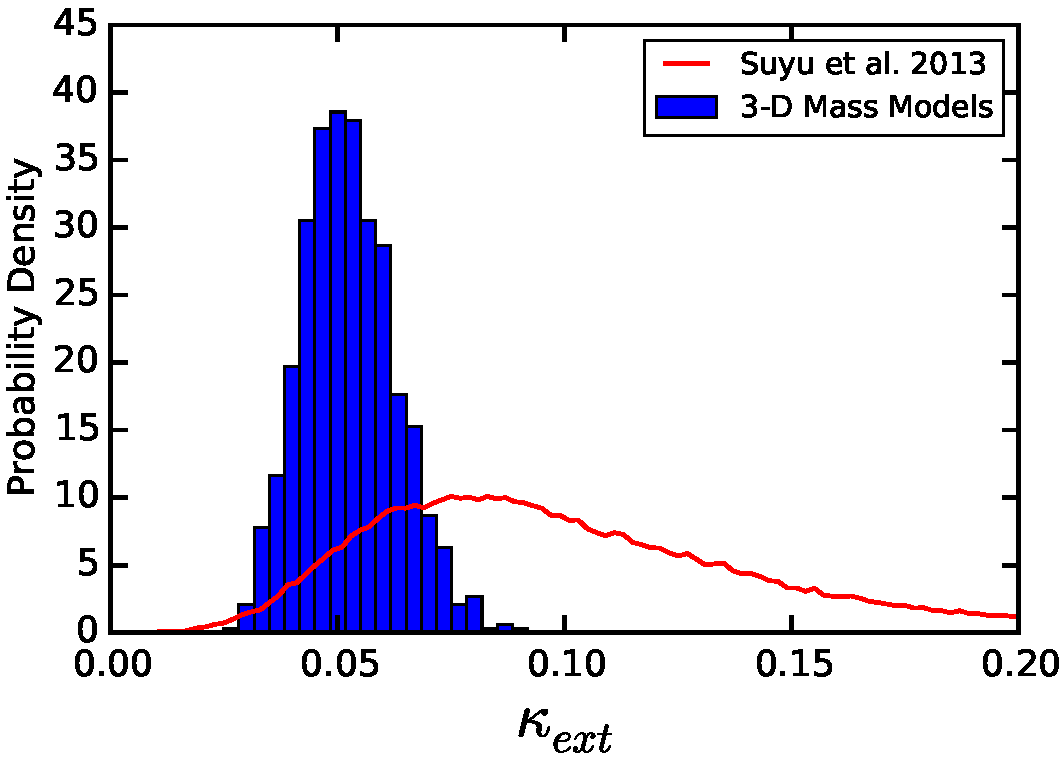
\includegraphics[width=\columnwidth]{suyu_kappa.pdf}
\caption{\label{fig:kappa} Probability distribution for the external convergence in the RXJ1131 field. The blue histogram shows the effective convergence computed directly from our 3-D mass models, accounting for measurement uncertainties and scatter in the relations used to assign masses to galaxies. The red curve shows the external convergence distribution derived using galaxy number counts from the Millennium simulation by \citet{Suyu13}. The peaks of the distributions match well. Because we build mass models for the specific, observed field, we obtain a $\sim 4$ times narrower distribution that effectively translates into a stronger prior on the Hubble constant.%
}
\end{center}
\end{figure}


Now that we have a quantity to assess the importance of indiviudal galaxies, we can apply this criterion to realistic mass models that have hundreds of ENV/LOS galaxies. This allows us to characterize which ENV/LOS galaxies produce the strong effects on the inferred Hubble constant. The perturbing ENV/LOS galaxies that produce strongest ENV/LOS effects can then be treated with more care (i.e., as ``main'' planes in our hybrid framework). The flexion shift criterion also gives us the ability to compare the mass models for different lens fields, in principle allowing us to select fields that do not have strong contributions as a ``gold sample'' of lenses for future surveys like LSST. 


To gain intuition about how the flexion shift applies to realistic beams, we first calculate the flexion shift for all of the perturbering ENV/LOS galaxies in the lens system RXJ1131, which has a source at redshift $z_{\rm{src}} = 0.658$ and a lens in a group at redshift $z_{\rm{lens}} = 0.2936$.  We adopt an Einstein radius of $R_E = 1.5''$, close to the measured value \citep{Suyu13} and also close to the peak of the observed distribution \citep{Sonnenfeld13}, and an ellipticity of $e=0.3$.  Figure \ref{fig:fieldrz} illustrates $\Delta_3 x$ values for galaxies in this field.  While $\Delta_3 x$ generally increases toward the lens, there is no single radial cut that can be used to determine the importance of a perturber because perturber mass and redshift must also be taken into account.  By following contours of constant $\Delta_3 x$, as illustrated in right-hand panel, we can determine the effective radial offset for the perturber if it were in the main lens plane. Since background perturbers are downweighted by ($1-\beta)^2$, they must have a smaller projected offset to have the same effect as if they were in the main lens plane. Perturbing galaxies in the foreground are slightly upweighted because the Einstein radius of a point mass perturber increases as we move it to lower redshift, which means that foreground galaxies can have a larger projected offset to have the same effect as if they were at the main lens redshift.

Figure \ref{fig:d3xhist} shows a histogram of all the $\Delta_3 x$ values for this field.  The flexion shifts range from $\sim 5 \times 10^{-3}$ arcseconds down to $<10^{-10}$ arcseconds, with background perturbers generally having smaller values than foreground perturbers or group members.  In the next section we consider the quantitative threshold for $\Delta_3 x$ needed to achieve desired accuracy and precision in lens model results.

We can also characterize values of the flexion shift for a wider range of fields.  Figure \ref{fig:allfields} shows $\Delta_3 x$ values for nine other multiply-imaged QSO fields from \citet{Wong11}.  The fields are all complex; there is not a simple radial cut that divides the sample into exact and tidal perturbers.  There is striking diversity in the strength of external effects.  There is no single number of galaxies that is guaranteed to be be the ``right'' number to include in lens models.  Each field must be considered on an individual basis.

While external convergence does not capture all LOS effects (it omits non-linearities in eq.\ \ref{eqn:full_mp}), it is a useful quantity for comparing to previous work. \citet{Suyu13} used the Millennium simulation along with galaxy number counts around RXJ1131 to estimate a prior probability distribution for the external convergence used to constrain the Hubble constant; their distribution is shown in red in Figure \ref{fig:kappa}. We compute the effective convergence (as defined in M14 and references therein) directly from our mass models for RXJ1131.  We consider many realizations that account for observational uncertainties and scatter in the relations used to assign masses to galaxies described above.  This yields a distribution of ``direct'' convergence calculations that is shown by the blue histogram in Figure \ref{fig:kappa}. We find that the peaks of the distributions match closely. However, our ``direct'' convergence calculations produce a tighter distribution by a factor of $\sim 4$. This is likely because we build mass models based on the observed beam for each individual lens rather than using statistical results from N-body simulations. The narrower distribution of external convergences translates into a stronger prior on measuring the Hubble constant.


While each field is unique, we expect that some fields will have stronger ENV/LOS contributions than others. One important factor may be whether the main lens galaxy is part of a group. To make a simple quantitative comparison, we add the flexion shifts ($\Delta_3 x$ values) in a given beam. The higher order effects due to flexion terms combine in a more complicated way (as the flexion is a tensor), but the simple sum gives an a good estimate of the importance of the ENV/LOS of the lens. If there are many nearby, massive perturbers then the sum will be large, implying a strong ENV/LOS contribution (such as HST14113 in Figure \ref{fig:allfields}). Conversely, in a sparser field the sum will be smaller (such as B0712). Figure \ref{fig:d3xsums} shows a histogram of the sums for our set of 23 lens field. While the sample size is not large, it is apparent that lenses that are members of a group tend to have stronger ENV/LOS contributions than those that are not.

\begin{figure}[!t]
\centering
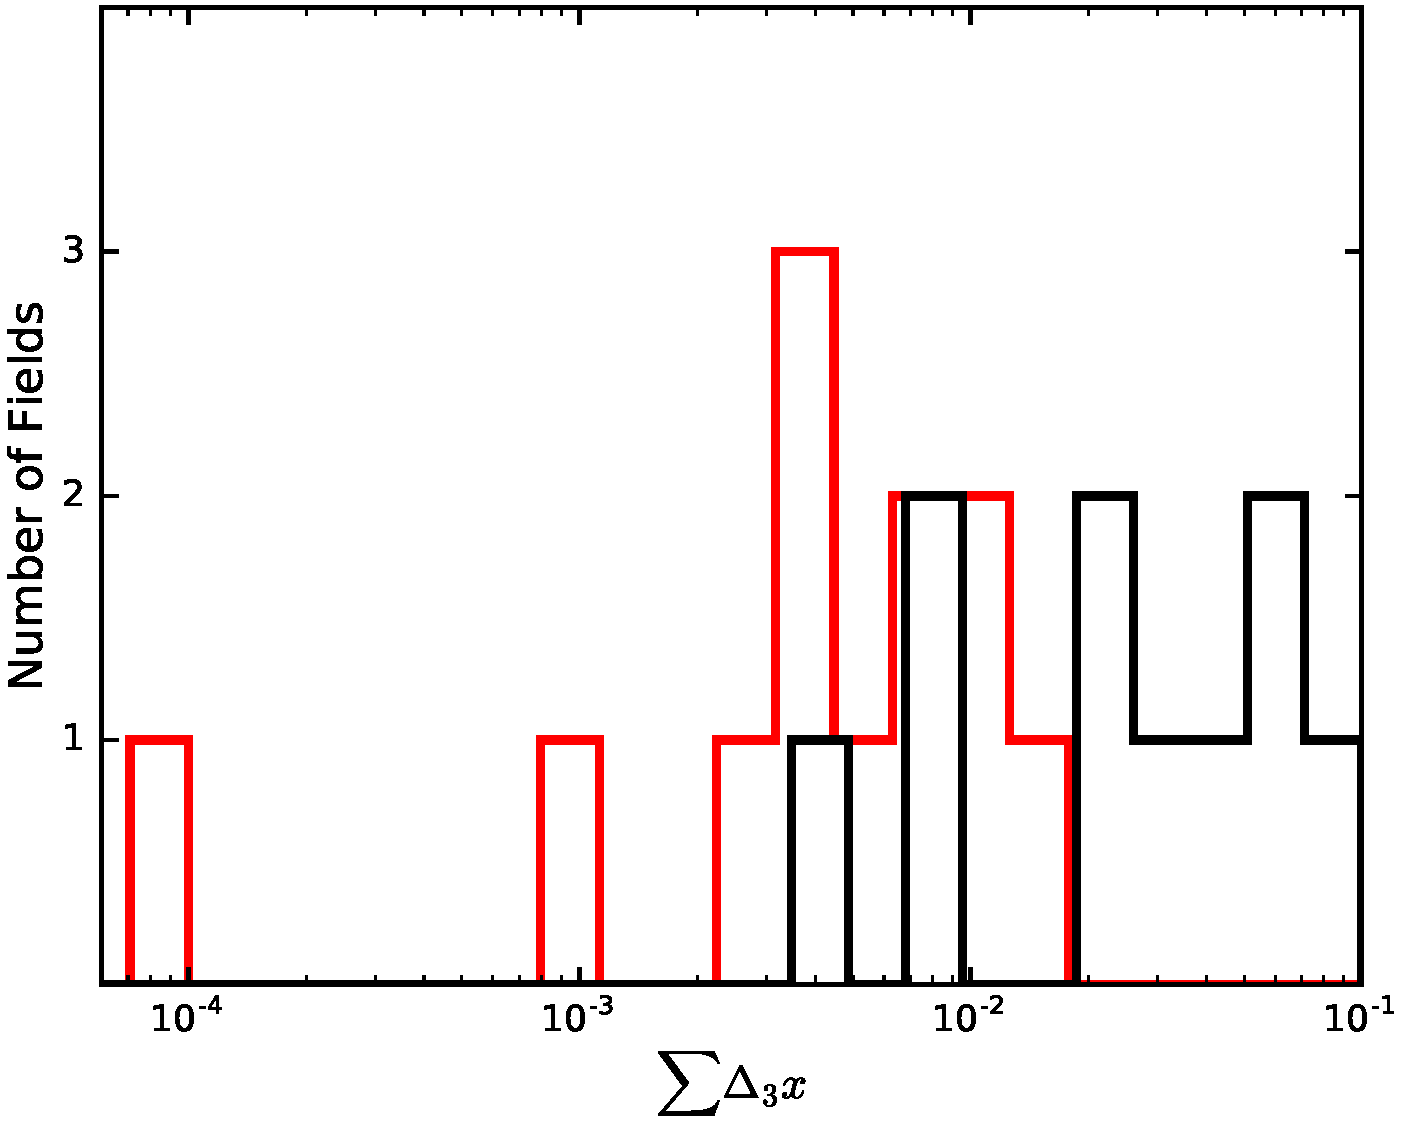
\includegraphics[width=\columnwidth]{d3xsums.pdf}
\caption{Distribution of ENV/LOS strengths for our sample of 3-D mass models. Beams for which the lens galaxy is a member of a group are shown in blue, while non-group lenses are shown in red. Lenses in groups typically have stronger ENV/LOS contributions than those that are not group memebers. However, there is substantial overlap so each field needs to be treated individually.}
\label{fig:d3xsums}
\end{figure}

%%%%%%%%%%%%%%%%%%%%%%%%%%%%%%%%%%%%%%%%
\subsection{Fitting Lens Observables}
\label{sec:fitting}
%%%%%%%%%%%%%%%%%%%%%%%%%%%%%%%%%%%%%%%%
Now that we have characterized our mass models, we consider whether different methods for treating ENV/LOS effects can reliably recover lens galaxy parameters and the Hubble constant. We generate mock lens observables using the full 3-D mass models in the simulations described in Section \ref{sec:observables}; throughout this analysis we combine results for 300 mock quad lenses with different source positions and azimuthal angles for the main lens galaxy. We then fit the mock lensing data using the three types of models discussed in Section \ref{sec:lensmodels}. We first test whether simple Lens-Only and Lens+Shear models can produce robust constraints on the Hubble constant. We then examine the 3-D Lens models to ascertain how well we do when we apply the tidal approximation to ENV/LOS galaxies. We also examine the parameter degeneracies in the 3-D Lens models.

\begin{figure*}[ht]
\begin{center}
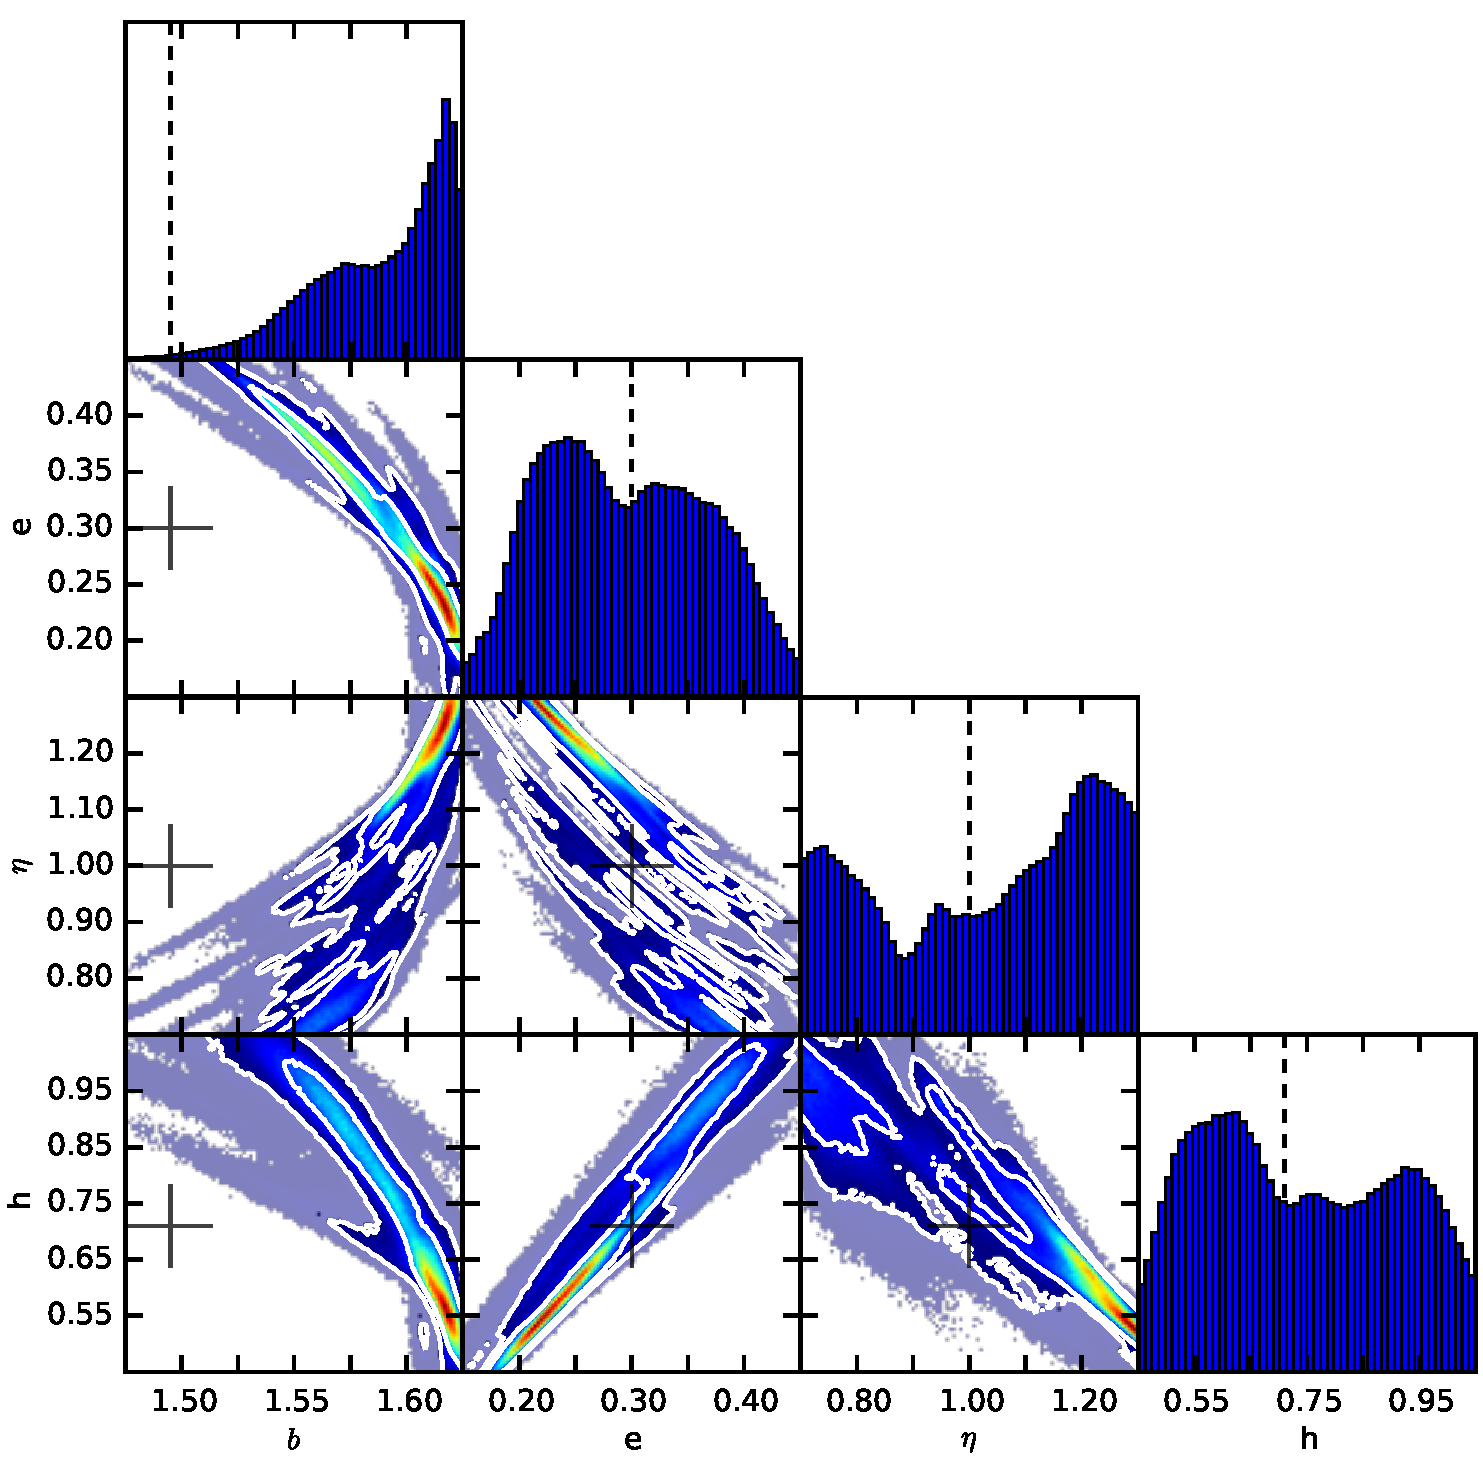
\includegraphics[width=1\textwidth]{all_none_1e-2.pdf}
\caption{\label{fig:none_triangle} Posterior distributions for model parameters from Lens-Only models fit to mock quad lenses in the field of RXJ1131. The true input values are marked with crosses in the contour plots and with a dashed line in the histograms. We combine MCMC results for 300 mock lenses with different source positions and azimuthal angles for the main lens galaxy.  Contours containing $68\%$ and $95\%$ of the MCMC trials are shown in white. Many of the parameters show significant biases and the distributions are often degenerate and multi-modal. These results suggest that ENV/LOS cannot be ignored. The recovered values of the Hubble constant have a scatter of $\sim 20\%$, more than an order of magnitude larger than our goal for ``Precision Lensing'' of $1\%$. The plotting ranges for corresponding parameters are the same as Figures \ref{fig:shear_triangle} and \ref{fig:los_triangle} to facilitate direct comparison.
}
\end{center}
\end{figure*}

We begin with Lens-Only models that do not explicitly account for any ENV/LOS effects. Figure \ref{fig:none_triangle} shows the recovered lens model parameters including the mass normalization (which is related to the Einstein radius; see eq.\ \ref{eqn:powerlaw}), ellipticity, power law index, and Hubble constant for the RXJ1131 field. The posterior distributions of the recovered lens parameters are broad and often multi-modal. All of the parameters show significant bias, and are not able to reproduce the input parameters. These results reiterate (not surprisingly) that ENV/LOS effects cannot be ignored.

\begin{figure*}[ht]
\begin{center}
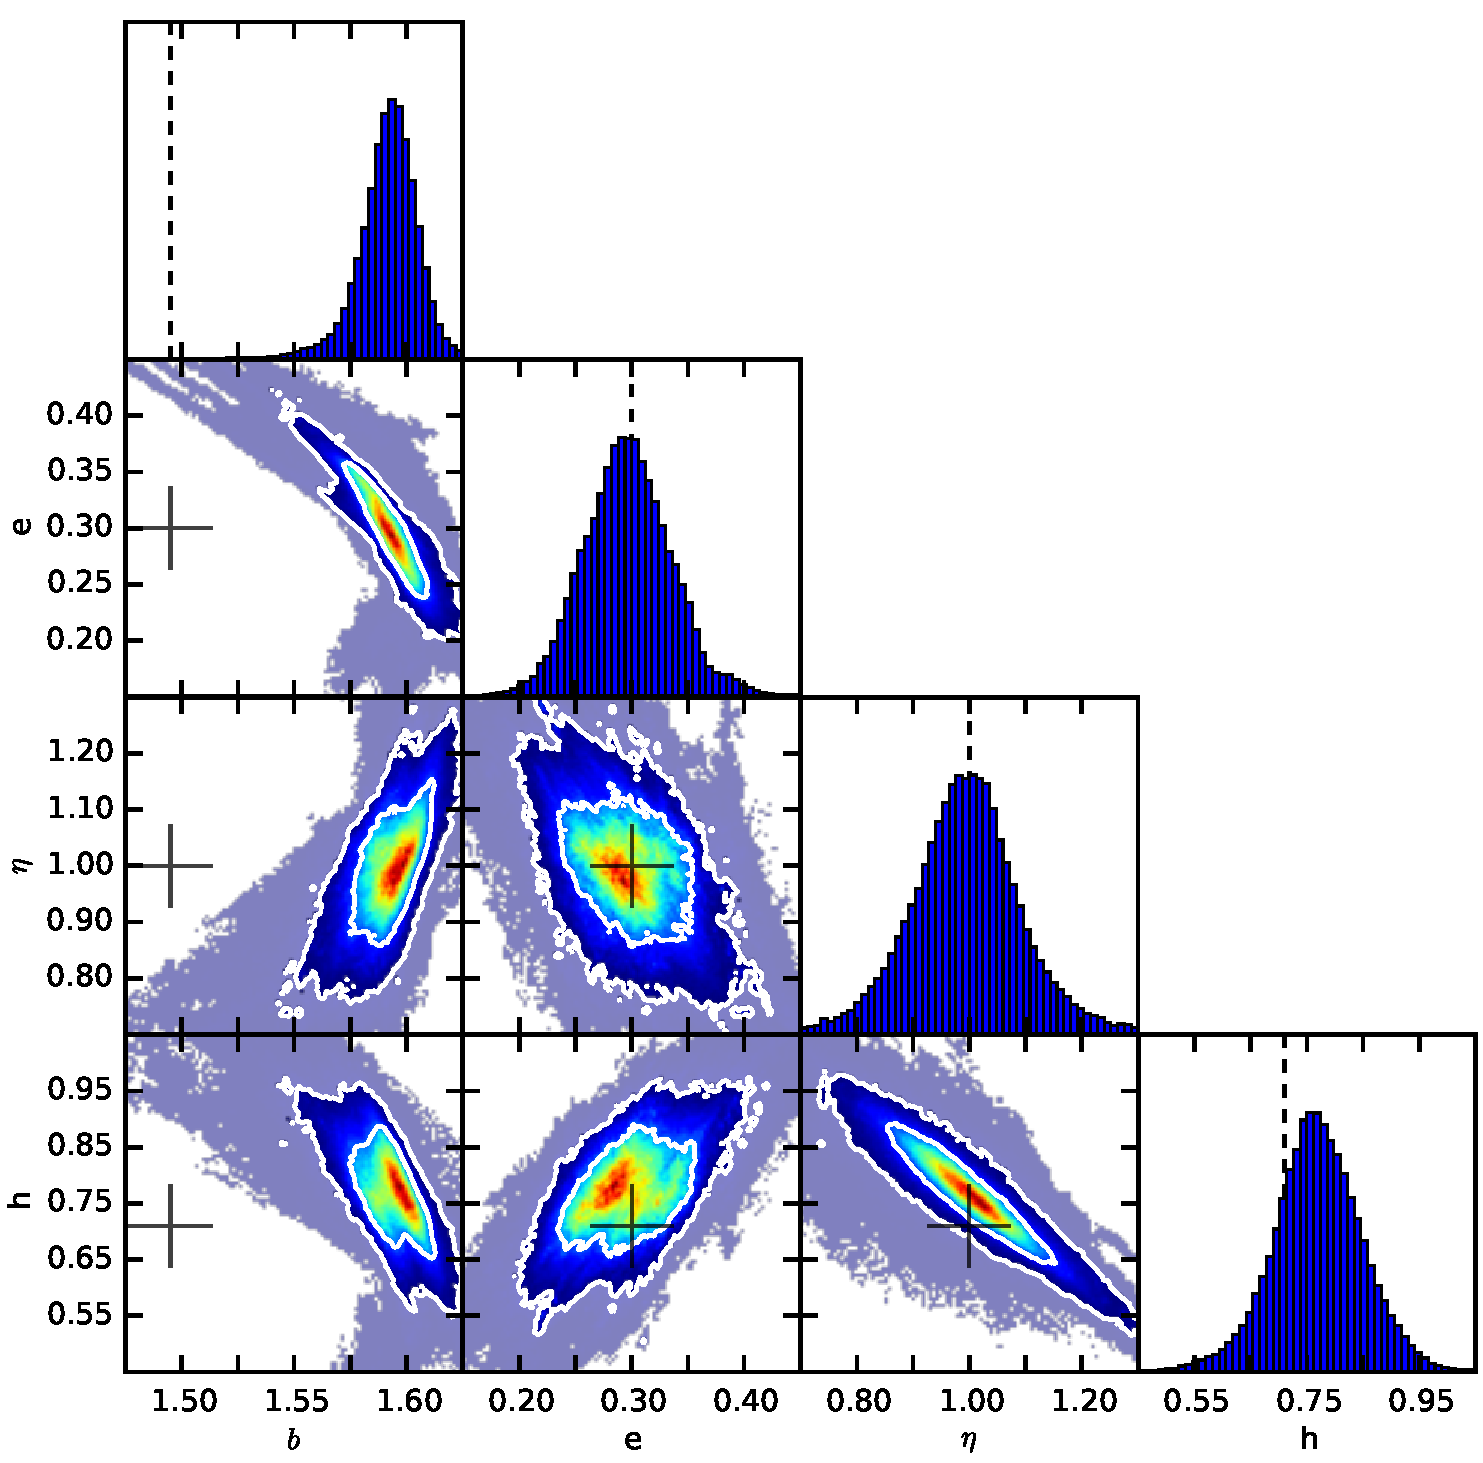
\includegraphics[width=1\textwidth]{all_shear_1e-2.pdf}
\caption{\label{fig:shear_triangle} Similar to Figure \ref{fig:none_triangle}, but for Lens+Shear models. Including an external shear dramatically improves the fits over ignoring the ENV/LOS, but the distribution of recovered parameters are non-Gaussian and may have multiple families of solutions. Many of the parameters show biases; most notably, the Einstein radius parameter ($b$) is strongly biased because Lens+Shear models do not explicitly include external convergence (such models must add external convergence in post-processing).  
}
\end{center}
\end{figure*}

Next we consider the Lens+Shear models. These models have two extra free parameters that can be used to capture some ENV/LOS effects. The results of the fits are shown in Figure \ref{fig:shear_triangle}. The posterior distributions of the recovered lens parameters are considerably tighter than for Lens-Only models. However, these models still have biases that are most dramatic in the Einstein radius and Hubble constant. The bias is associated with external convergence: the total mass in the simulated lenses includes contributions from the environment and LOS; if we assign all of that mass to the main lens galaxy (as in Lens+Shear and Lens-Only models), we overestimate the galaxy's mass and Einstein radius.  In the traditional approach, external convergence must be included through post-processing \citep{Collett13, Suyu10}. 

\begin{figure}[ht]
\centering
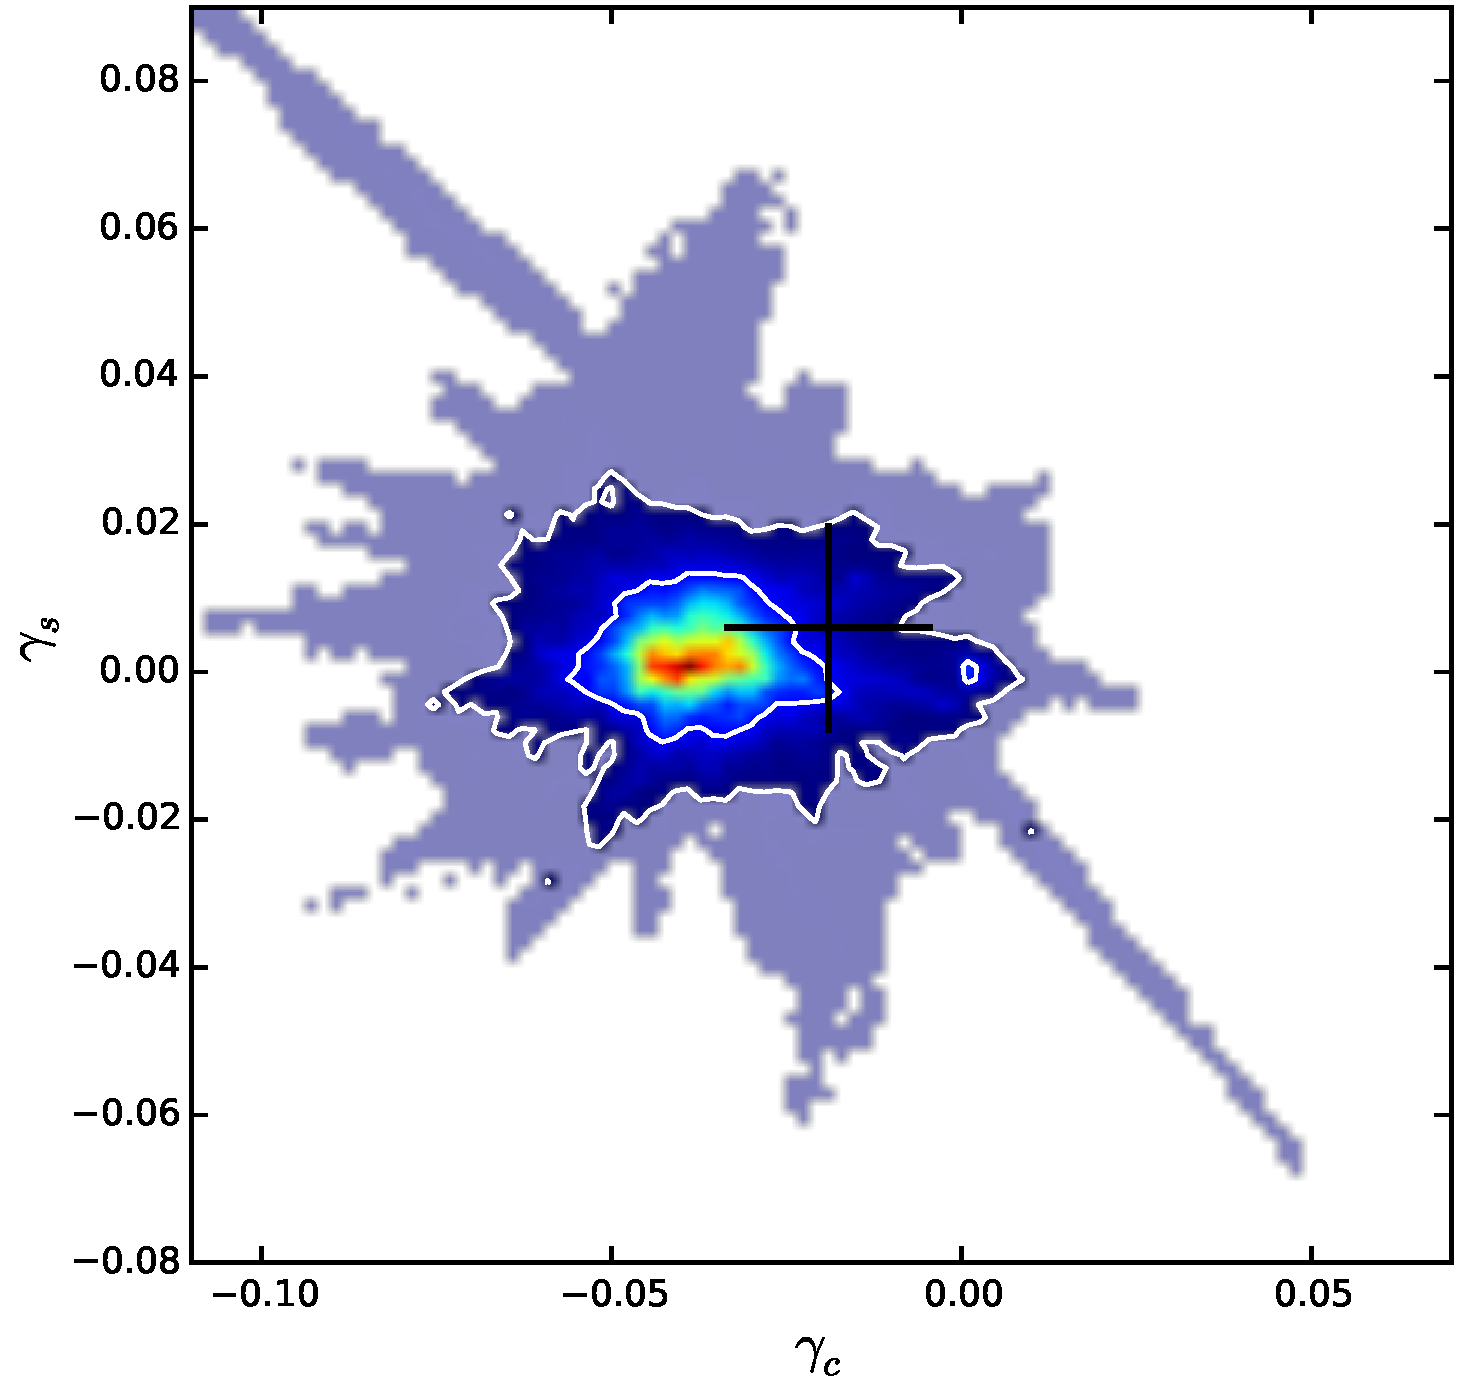
\includegraphics[width=\columnwidth]{shear_offset.pdf}
\caption{Marginalized posterior distribution of fitted external shear values from the Lens+Shear models. $68\%$ and $95\%$ contours are shown in white. The effective shear calculated from the input 3-D mass model is shown with an orange cross. The peak of the distribution from the MCMC models is $\sim 2.5 \sigma$ away from the truth, similar to what was found by \citet{Wong11}. The offset appears to be inherent to the lens modelling process, possibly due to non-linear effects from foreground perturbing galaxies.}
\label{fig:shear_compare}
\end{figure}

\citet{Wong11} found that fitted shear parameters from the Lens+Shear models did not always match the shears computed directly from 3-D mass models in real lenses, including RXJ1131. We reexamine this result using our controlled simulations. Figure \ref{fig:shear_compare} compares the distributed of fitted shear parameters with the known value of the effective shear for this ENV/LOS. The fitted shear parameters disagree with the true effective shear at the $\sim 2.5\sigma$ level, broadly consistent with the results found in \citet{Wong11}. While a deeper analysis of the difference is beyond the scope of this work, the results in Figure \ref{fig:shear_compare} suggest that the offsets found by \citet{Wong11} are associated with the lens modeling procedure; they may arise because the fitted shear is attempting to account for non-linear effects due to foreground perturbing galaxies.

\begin{figure*}[ht]
\begin{center}
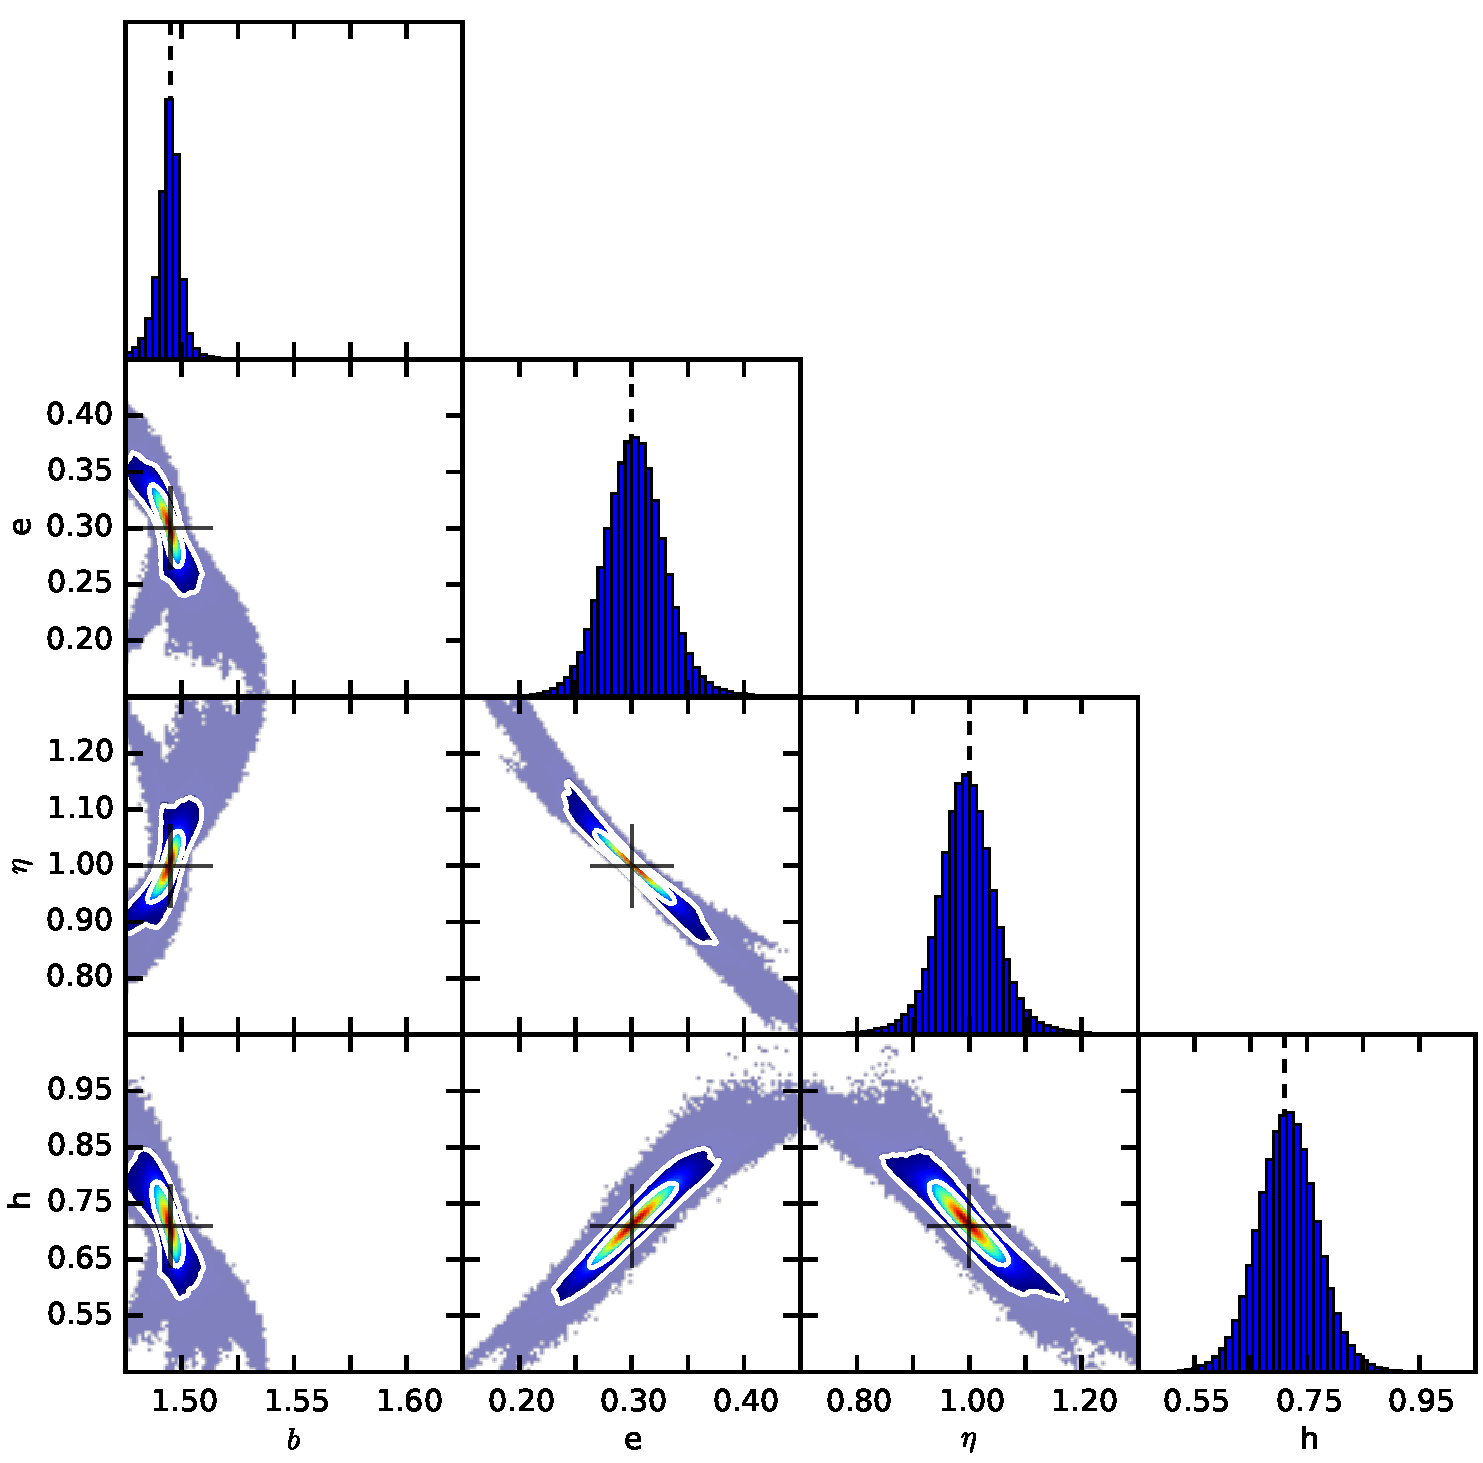
\includegraphics[width=1\textwidth]{all_los_1e-2.pdf}
\caption{\label{fig:los_triangle} Similar to Figure \ref{fig:none_triangle}, but for 3-D Lens models. Here all perturbing galaxies are treated with the 3-D tidal approximation.  There is no bias in the recovered parameters, implying that omitting higher order terms will not bias our measurements of the Hubble constant. The scatter in the recovered parameters is much smaller than that of the Lens+Shear and Lens-Only models. However, there are still strong correlations between ellipticity, the power law index, and the Hubble constant. This is a manifestation of the lens profile degeneracy \citep{Kochanek02}. %
}
\end{center}
\end{figure*}

Lastly, we consider our 3-D lens models. We initially treat all perturbing galaxies in the tidal approximation. This allows us to disentangle the non-linear effects, which are included in our models because we use the same mass model that was used to generate the lensing observables, and higher-order terms, which are included when generating the lens observables (see Section \ref{sec:observables}), but not in the fits. 
Figure \ref{fig:los_triangle} shows posterior distributions of the recovered lens parameters and Hubble constant. There is no bias in any of the parameters recovered from these models. Our 3-D Lens models avoid the biases seen in other models because, rather than treating shear and convergence separately, we build a physical model and then extract both shear and convergence self-consistently. We favor this approach because shear and convergence arise from the same underlying mass distribution and are therefore not independent.

However, there are strong correlations among the recovered ellipticity, power law index, and Hubble constant for our 3-D lens models. These correlations involving the Hubble constant are associated with the ``lens profile degeneracy'':  there can be a range of density profiles that all yield a good fit but lead to different values for $h$.  \citet{Kochanek02} shows that to lowest order the degeneracy is characterized by the scaling $h \propto 1 - \langle \kappa \rangle$ where $\langle \kappa \rangle$ is the average convergence from the main lens in the annulus between the image positions.  If we assume that the image annulus is narrow and centered on the Einstein radius, we can evaluate the angle average as
\begin{equation}
\langle \kappa \rangle = \frac{1}{2 \pi} \int_{0}^{2 \pi} \kappa(R_E, \theta) d \theta.
\end{equation}
With our power law model (eq.\ \ref{eqn:powerlaw}), we can evaluate the integral by making a Taylor series expansion in the ellipticity and using
\begin{equation}\label{eqn:e-series}
\int_0^{2 \pi} \frac{d \theta}{ (1 - 2 e \cos^2(\theta) + e^2\cos^2(\theta))^{1 - \eta / 2}} \approx 1 + e  - \frac{ e \eta}{2}.
\end{equation}
For typical parameter values of interest, we find numerically that this approximation is good to $\sim1\%$.  Then we can approximate the average convergence at the Einstein radius as
\begin{equation}\label{eqn:kappa-avg}
\langle \kappa \rangle \approx \frac{1}{2} \eta  (1 - e)^{2 - \eta} \left(1 +  e - \frac{e \eta }{2}\right).
\end{equation}
We test this analysis by plotting $h/(1-\langle\kappa\rangle)$ in Figure \ref{fig:scaled_triangle}.  Most of the correlation of $h$ with $\eta$ and $e$ has been accounted for.  Remaining correlations are likely due to higher order terms in the expression for $h$ as a function of profile parameters \citep{Kochanek02} and the Taylor series expansion in equation \ref{eqn:e-series}.

\begin{figure*}[ht]
\begin{center}
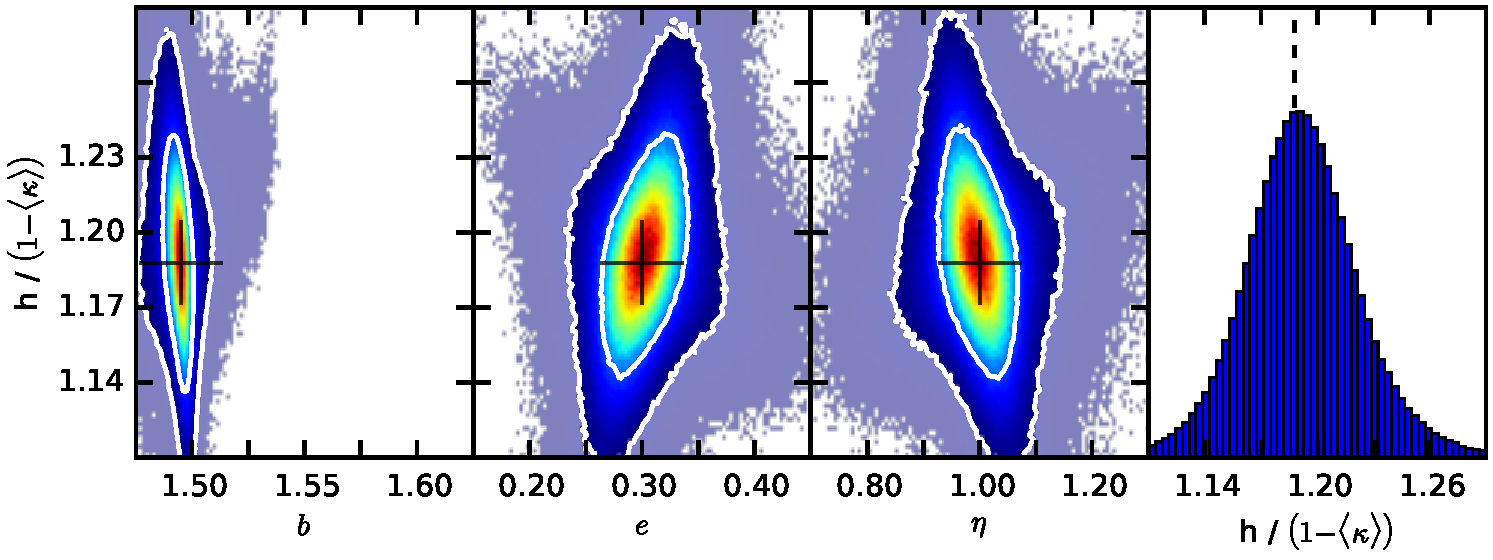
\includegraphics[width=1\textwidth]{los_scaled_h.pdf}
\caption{\label{fig:scaled_triangle} Recovered parameter distributions for 3-D Lens models (q.v.\ Fig.\ \ref{fig:los_triangle}), but now with the Hubble constant, $h$, scaled to account for the lens profile degeneracy.  We approximate the average convergence at the Einstein radius using equation \ref{eqn:kappa-avg}. The correlations among the Hubble constant, ellipticity, and power law index are mostly removed. The residual correlations are likely due to higher order terms in the expression for $h$ \citep{Kochanek02} and the Taylor series expansion for $\langle \kappa \rangle$.%
}
\end{center}
\end{figure*}

The fact that these correlations are seen in our 3-D lens models suggests that the ENV/LOS does not break the lens profile degeneracy. This is consistent with the idea that ENV/LOS effects are produced by structure on much larger spatial scales than is relevant for the lens profile degeneracy \citep{Xu15,Schneider13}. The lens profile must be broken instead with kinematic information \citep[e.g.][]{Suyu13} or with extended source modeling \citep{Suyu12}.

Our next goal is to determine when it is valid to use the tidal approximation.  We want to find a sweet spot that speeds up the modeling without introducing systematic uncertainties that are larger than the measurement uncertainties.  Figure \ref{fig:RXJ1131} shows results from 3-D Lens model fits with different cuts on the flexion shift, $\Delta_3 x$.  Each point on the horizontal axis corresponds to a different \emph{threshold} for $\Delta_3 x$: galaxies with larger flexion shifts are treated exactly, while galaxies with smaller values are treated with the tidal approximation.  (Note that the threshold \emph{decreases} from left to right in the plot; at a given point, galaxies to the left are exact perturbers while galaxies to the right are tidal perturbers.)  The error bars mark the $16^{th}$ and $84^{th}$ percentiles of the posterior distribution for the lens model parameters.  Our modeling uses MCMC methods to obtain posterior distributions, so the errorbars correspond to marginalized single-parameter posteriors.

The first result from Figure \ref{fig:RXJ1131} is that 3-D Lens models do not show any bias in key parameters, even if all of the ENV/LOS galaxies are treated in the tidal approximation, at least for the RXJ1131 field. The scatter in model parameters decreases a little as the $\Delta_3 x$ threshold is reduced and the strongest perturbers are incorporated into the model explicitly.  We believe that it is worthwhile to set a conservative threshold of $\Delta_3 x \sim 10^{-4}$ arcseconds (i.e., 1.5 dex smaller than our astrometric uncertainties), which amounts to including the strongest 10--15 perturbers explicitly as main planes. The computational complexity of the full multi-plane lens equation scales as $\sim N^2$, the reduction from $\sim 300$ galaxies to treating all but 10--15 using the tidal approximation produces an improvement in the performance by a factor of 400--900.

However, the Lens-Only and Lens+Shear models do show a bias, as mentioned above. Introducing a few of the strongest perturbers (i.e., moving to the right in the figure) means that we begin to explicitly include the most important ENV/LOS galaxies. Thus as we move to the right in the figure, the need for an ``external'' convergence is no longer necessary because it already included in the models, which in turn reduces the bias in the recovered parameters.  In principle, there is a point at which the sources of convergence are properly accounted for and the bias is removed.  In practice, that point is not easy to determine \emph{a priori}.  Going to very small values of $\Delta_3 x$ (i.e., far to the right in the figure) actually leads to a negative bias.  This is because Lens-Only and Lens+Shear models do not include the void correction discussed in Section \ref{sec:voids}.  Apparently the void correction is approximately 2\% in the Einstein radius for the RXJ1131 field.


\begin{figure}[ht]
\begin{center}
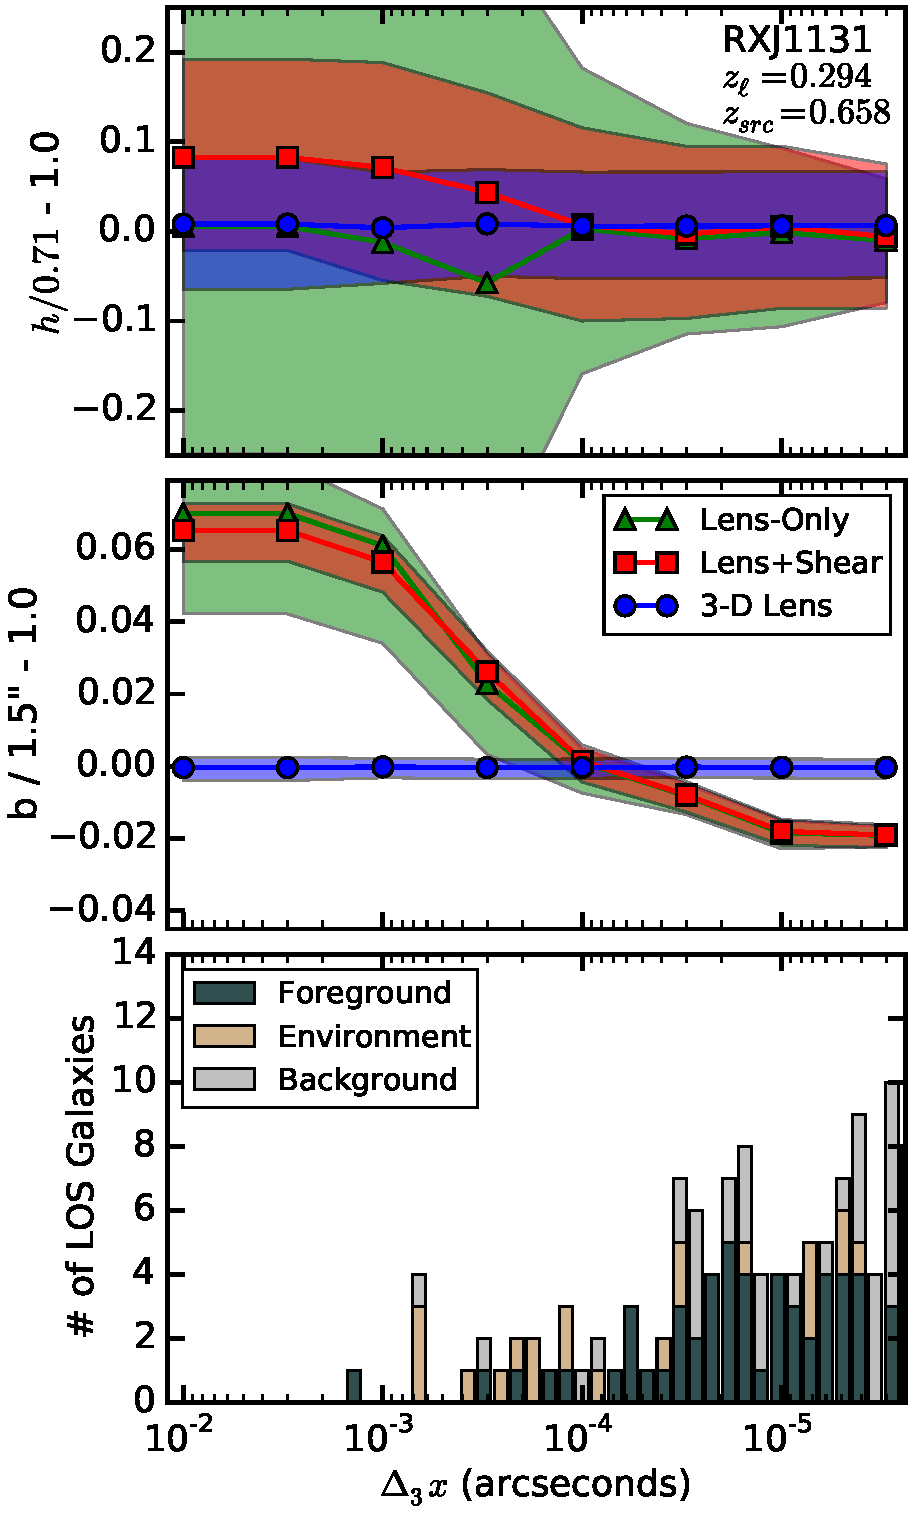
\includegraphics[width=1\columnwidth]{new_RXJ1131_reallos.pdf}
\caption{\label{fig:RXJ1131} Results for lens models with different thresholds for the tidal approximation, using the RXJ1131 field.  For a given value of $\Delta_3 x$, we run models in which all perturbing galaxies with a larger value of the flexion shift (i.e., those toward the left in the bottom panel) are treated exactly, while perturbing galaxies with a smaller value of the flexion shift (i.e., those toward the right) are treated with the tidal approximation.  Starting at the left, all perturbers are tidal (as in Figs.\ \ref{fig:none_triangle},  \ref{fig:shear_triangle}, and \ref{fig:los_triangle}); moving to the right increases the number of perturbers that are treated explicitly instead.  The top panel shows the median and 68\% confidence interval for the Hubble constant recovered from 3-D Lens models (blue), Lens+Shear models (red), and Lens-Only models (green). The scatter is driven by the lens profile degeneracy.  The middle panel shows similar results for the Einstein radius parameter. Lens-Only and Lens+Shear models tend to be biased because of external convergence effects which are typically added in post-processing. For RXJ1131, this accounts for a $7\%$ correction, consistent with the peak of the distribution shown in Figure \ref{fig:kappa}. As we include more galaxies exactly, moving to the right of the plot, the bias begins to disappear because we are taking into account more of the convergence explicitly. However, as we take many of the ENV/LOS galaxies into account exactly, the Lens-Only and Lens+Shear models dip below the truth. This is due to the smooth mass correction for voids which is not included in the Lens-Only and Lens+Shear models. Our simulation results suggest that the void correction is $\sim 2\%$ for RXJ1131.
}
\end{center}
\end{figure}

So far, we have presented results for a single lens field.  In order to understand whether our conclusions are general, we need to examine how ENV/LOS effects vary from one lensing field to another. One simple test is to compare models that use the same fiducial main lens galaxy ($R_E = 1.5\arcsec$ and $e=0.3$) but different fields.  Figure \ref{fig:B0712} shows results from simulations using the field of B0712+472 (hereafter B0712; \citealt{Jackson98}).  The trends are similar to what we saw for RXJ1131 in Figure \ref{fig:RXJ1131}, but the deviations are somewhat smaller here because the ENV/LOS effects are not as strong in this field (as we saw in Section \ref{sec:Environments}).  The correction due to voids is larger for B0712 at $\sim4\%$. Therefore, the qualitative trends of our results appear to be robust, but the quantiative differences indicate that each lens field needs to be treated on an individual basis.

\begin{figure}[t]
\begin{center}
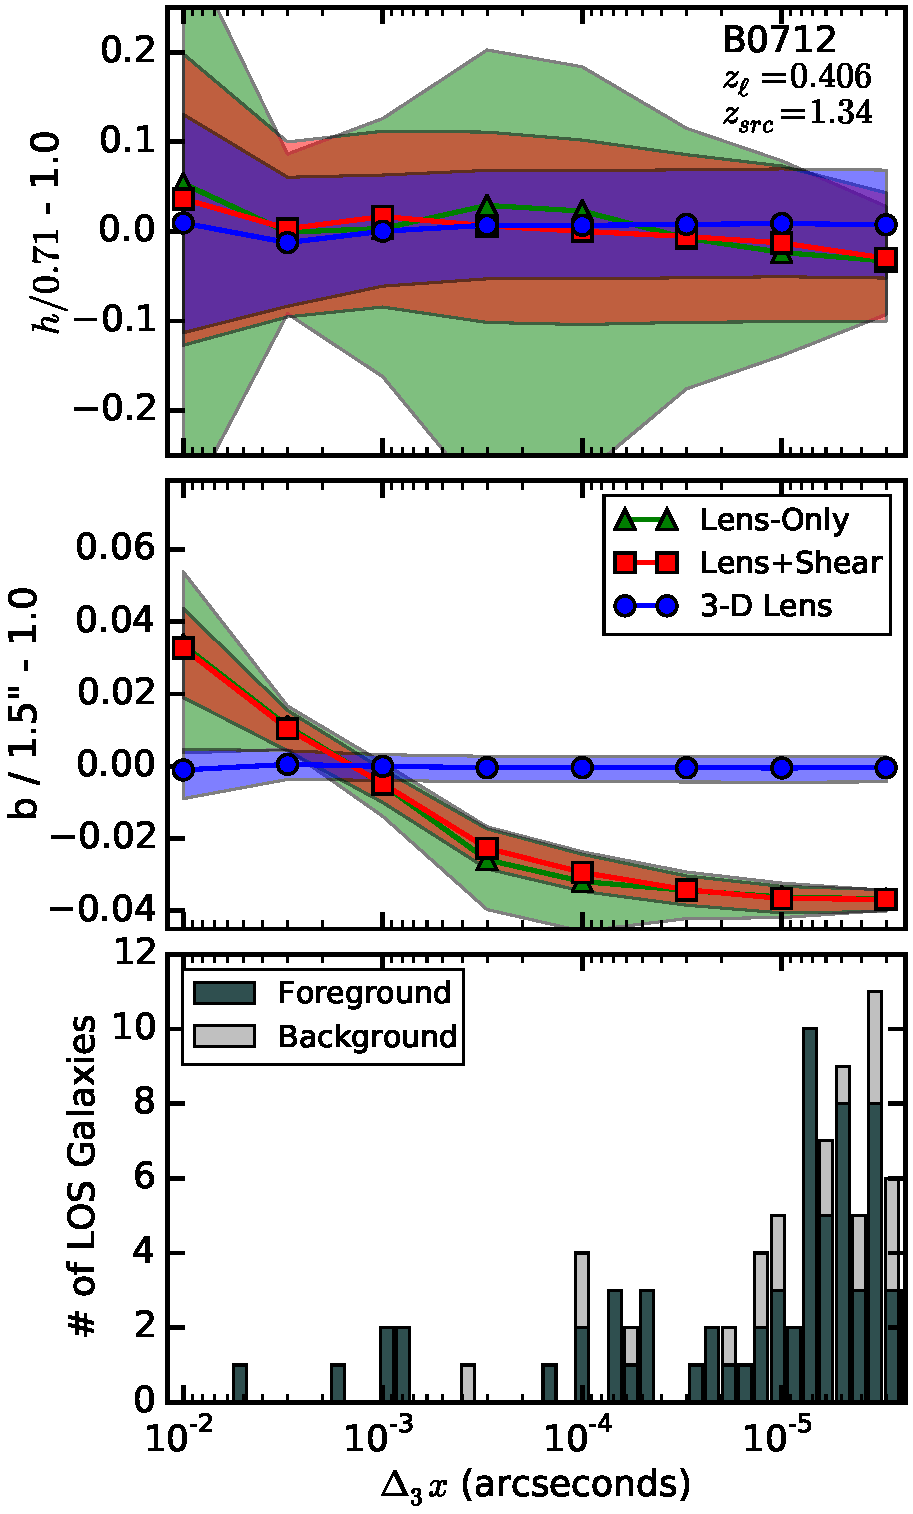
\includegraphics[width=\columnwidth]{new_B0712_reallos.pdf}
\caption{\label{fig:B0712} Similar to Figure \ref{fig:RXJ1131}, but for the B0712 field.  This lens is not in a group in our mass models, but it does have a group of galaxies along the LOS.  The qualitative trends from the ENV/LOS effects are similar to what we saw for RXJ1131, but the quantitative details differ. The correction for external convergence (seen at the farthest left point) is smaller for B0712, at $\sim 4\%$, than what we saw for RXJ1131 at $\sim 7\%$. This is consistent with the results from Figure \ref{fig:d3xsums} that group lenses typically have stronger ENV/LOS effects than non-group lenses. The correction for the smooth mass density (e.g., voids; inferred from the farthest right point) is larger for B0712 , at $\sim 4\%$, than for RXJ1131 which only had a correction of $2 \%$.
}
\end{center}
\end{figure}

In this analysis we have placed the same lens galaxy in different 3-D mass models to see how the ENV/LOS effects vary.  The complementary step is to fix the 3-D model and vary the main lens galaxy to understand how that changes the sensitivity to ENV/LOS effects.

%%%%%%%%%%%%%%%%%%%%%%%%%%%%%%%%%%%%%%%%
\subsection{What Lens Properties Yield the Strongest Constraints on Cosmology?}
\label{sec:ImageConfigs}
%%%%%%%%%%%%%%%%%%%%%%%%%%%%%%%%%%%%%%%%

In our final set of simulations, we choose one ENV/LOS mass model (for the RXJ1131 field) and test how the constraints on the Hubble constant change when we vary the parameters of the main lens galaxy and the position of the source behind the lens.

One important parameter of the main lens galaxy is the ellipticity. Figure \ref{fig:ecompare} compares results from simulations with different values of $e$.  As the ellipticity increases, the scatter in the recovered Hubble constant decreases.
The image configurations of very asymmetric lens galaxies can only be produced for a smaller range of lens models, leading to stronger constraints on both the ellipticity and the power law index.  Since those parameters are correlated with the Hubble constant through the lens profile degeneracy, reducing the range of $e$ and $\eta$ leads to a narrower range for $h$ as well.

\begin{figure*}
\begin{center}
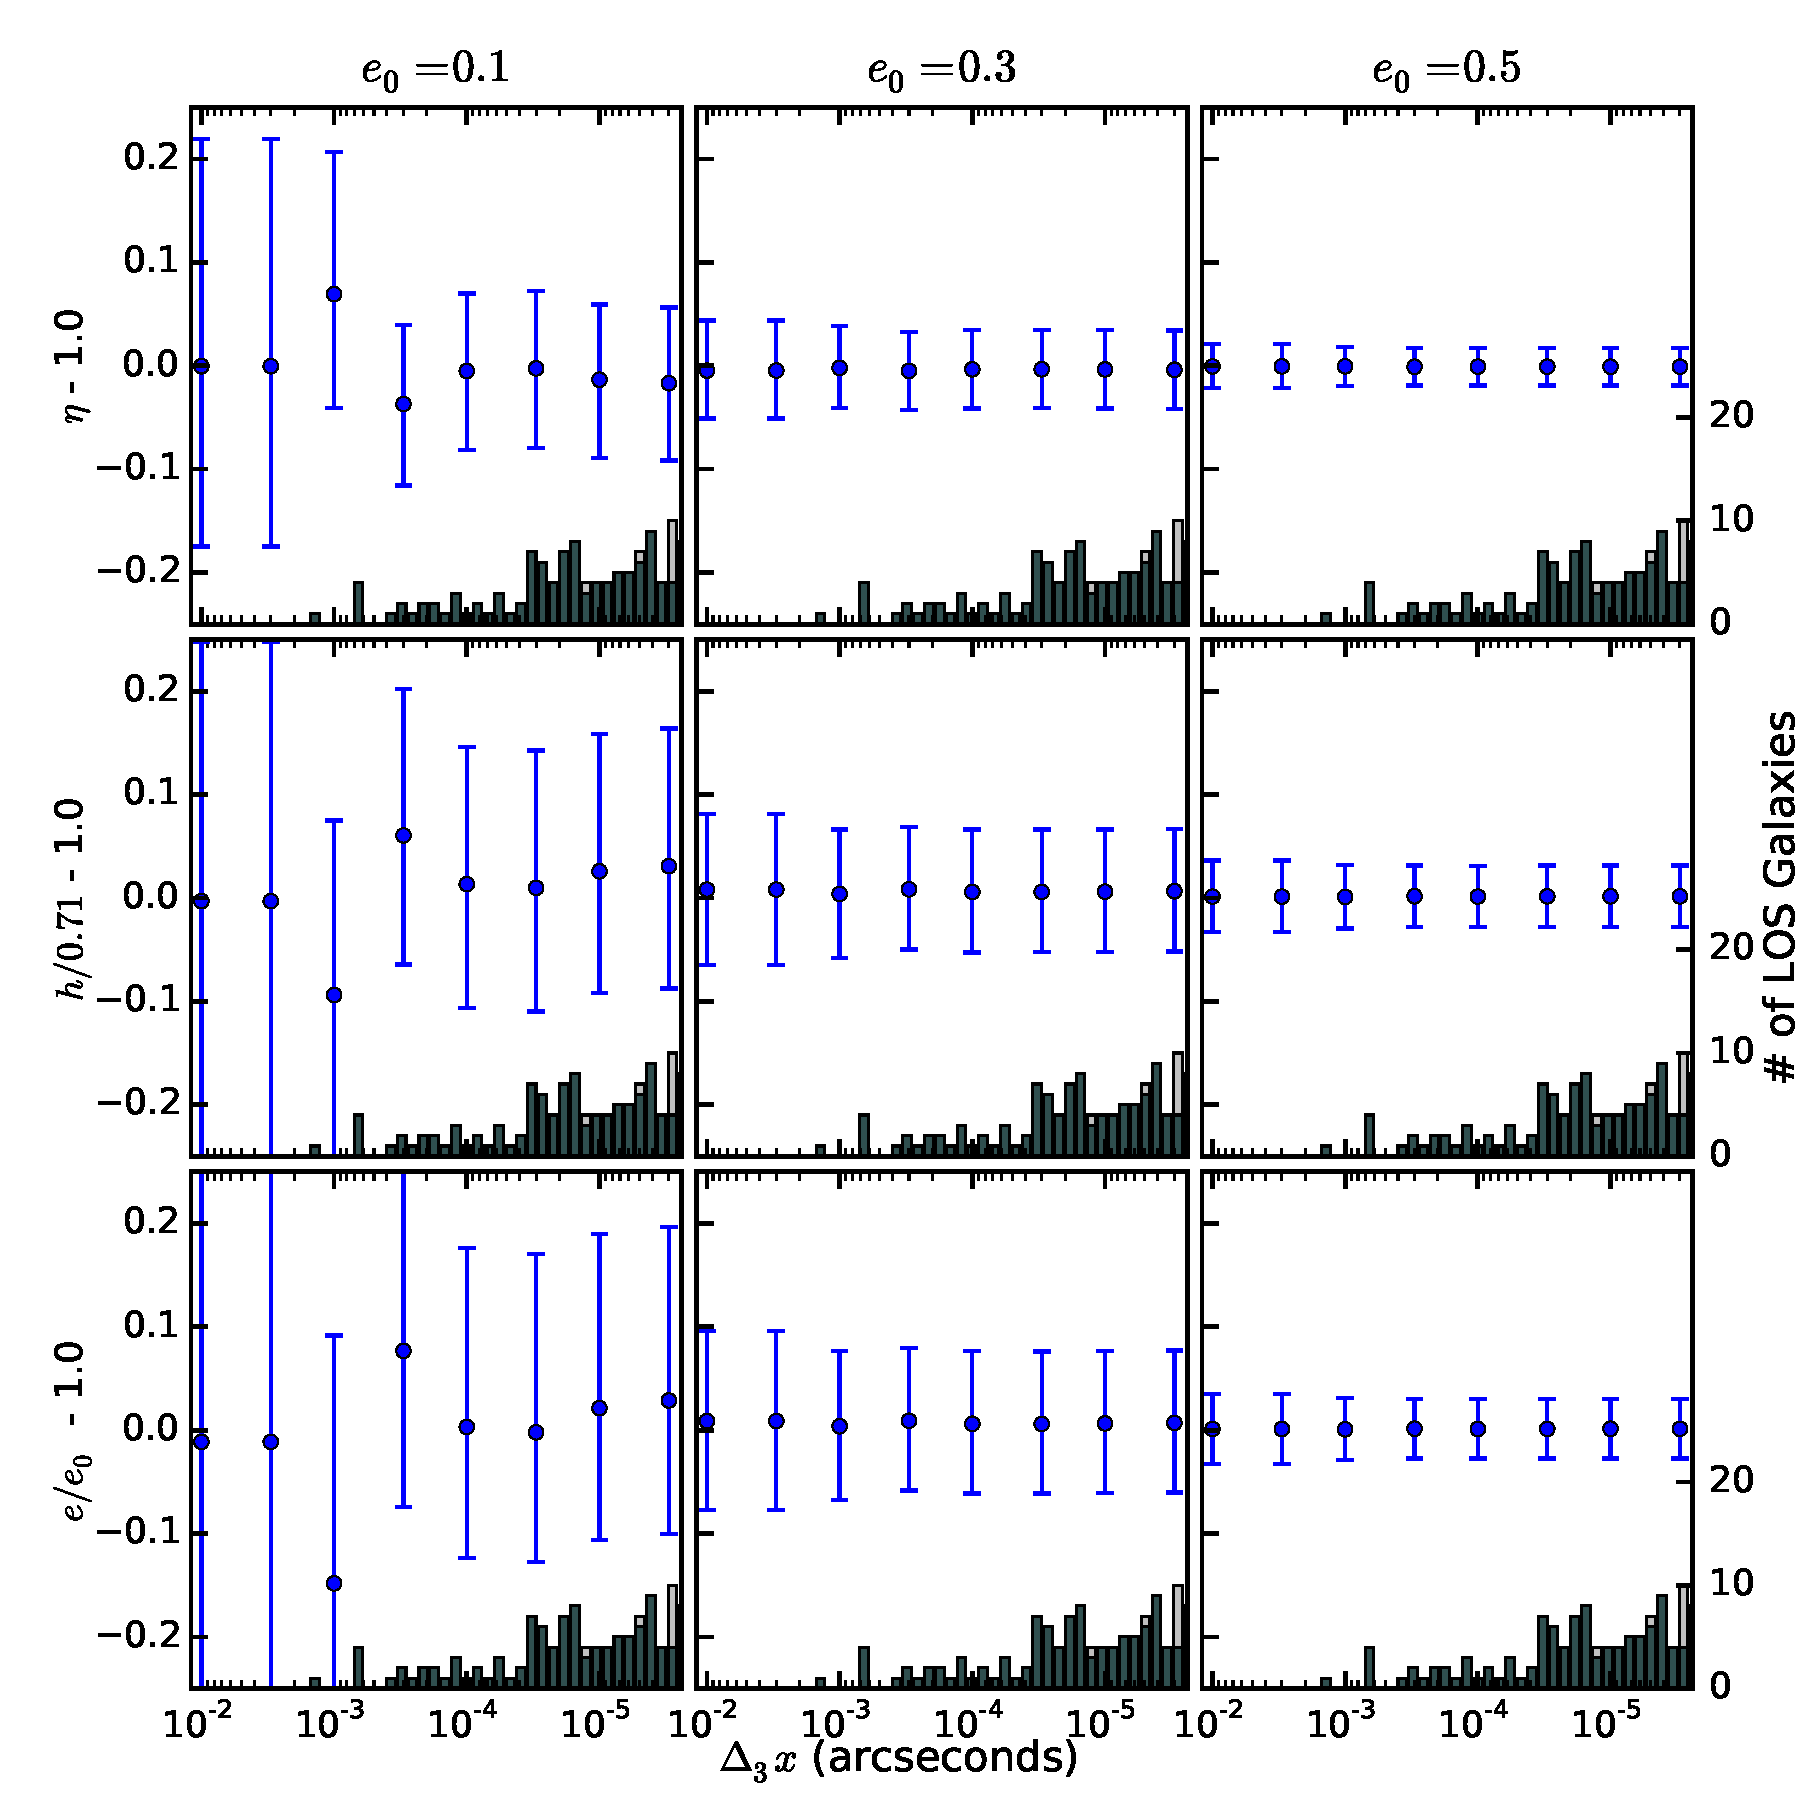
\includegraphics[width=1\textwidth]{ecompare.pdf}
\caption{\label{fig:ecompare} Recovered model parameters for main lens galaxies with different ellipticities, using the RXJ1131 field. The columns correspond to $e = 0.1,0.3,0.5$ from left to right. Systems with larger $e$ have less scatter in the power law index, $\eta$, and the Hubble constant, $h$. Elongated lenses tend to produce more asymmetric image configurations. More asymmetric image configurations span a wider range of radii and provide strong constraints on the ellipticity, breaking the lens profile degeneracy and producing tighter constraints on the Hubble constant.%
}
\end{center}
\end{figure*}

A second key parameter of the main lens galaxy is the Einstein radius. Figure \ref{fig:recompare} shows model results for different values of the Einstein radius parameter $b$.  As the Einstein radius increases, the constraints on the Hubble constant get stronger. Lenses with large Einstein radii produce stronger constraints on the ellipticity limiting the lens profile degeneracy, yielding a tighter distribution on the Hubble constant.

\begin{figure*}
\begin{center}
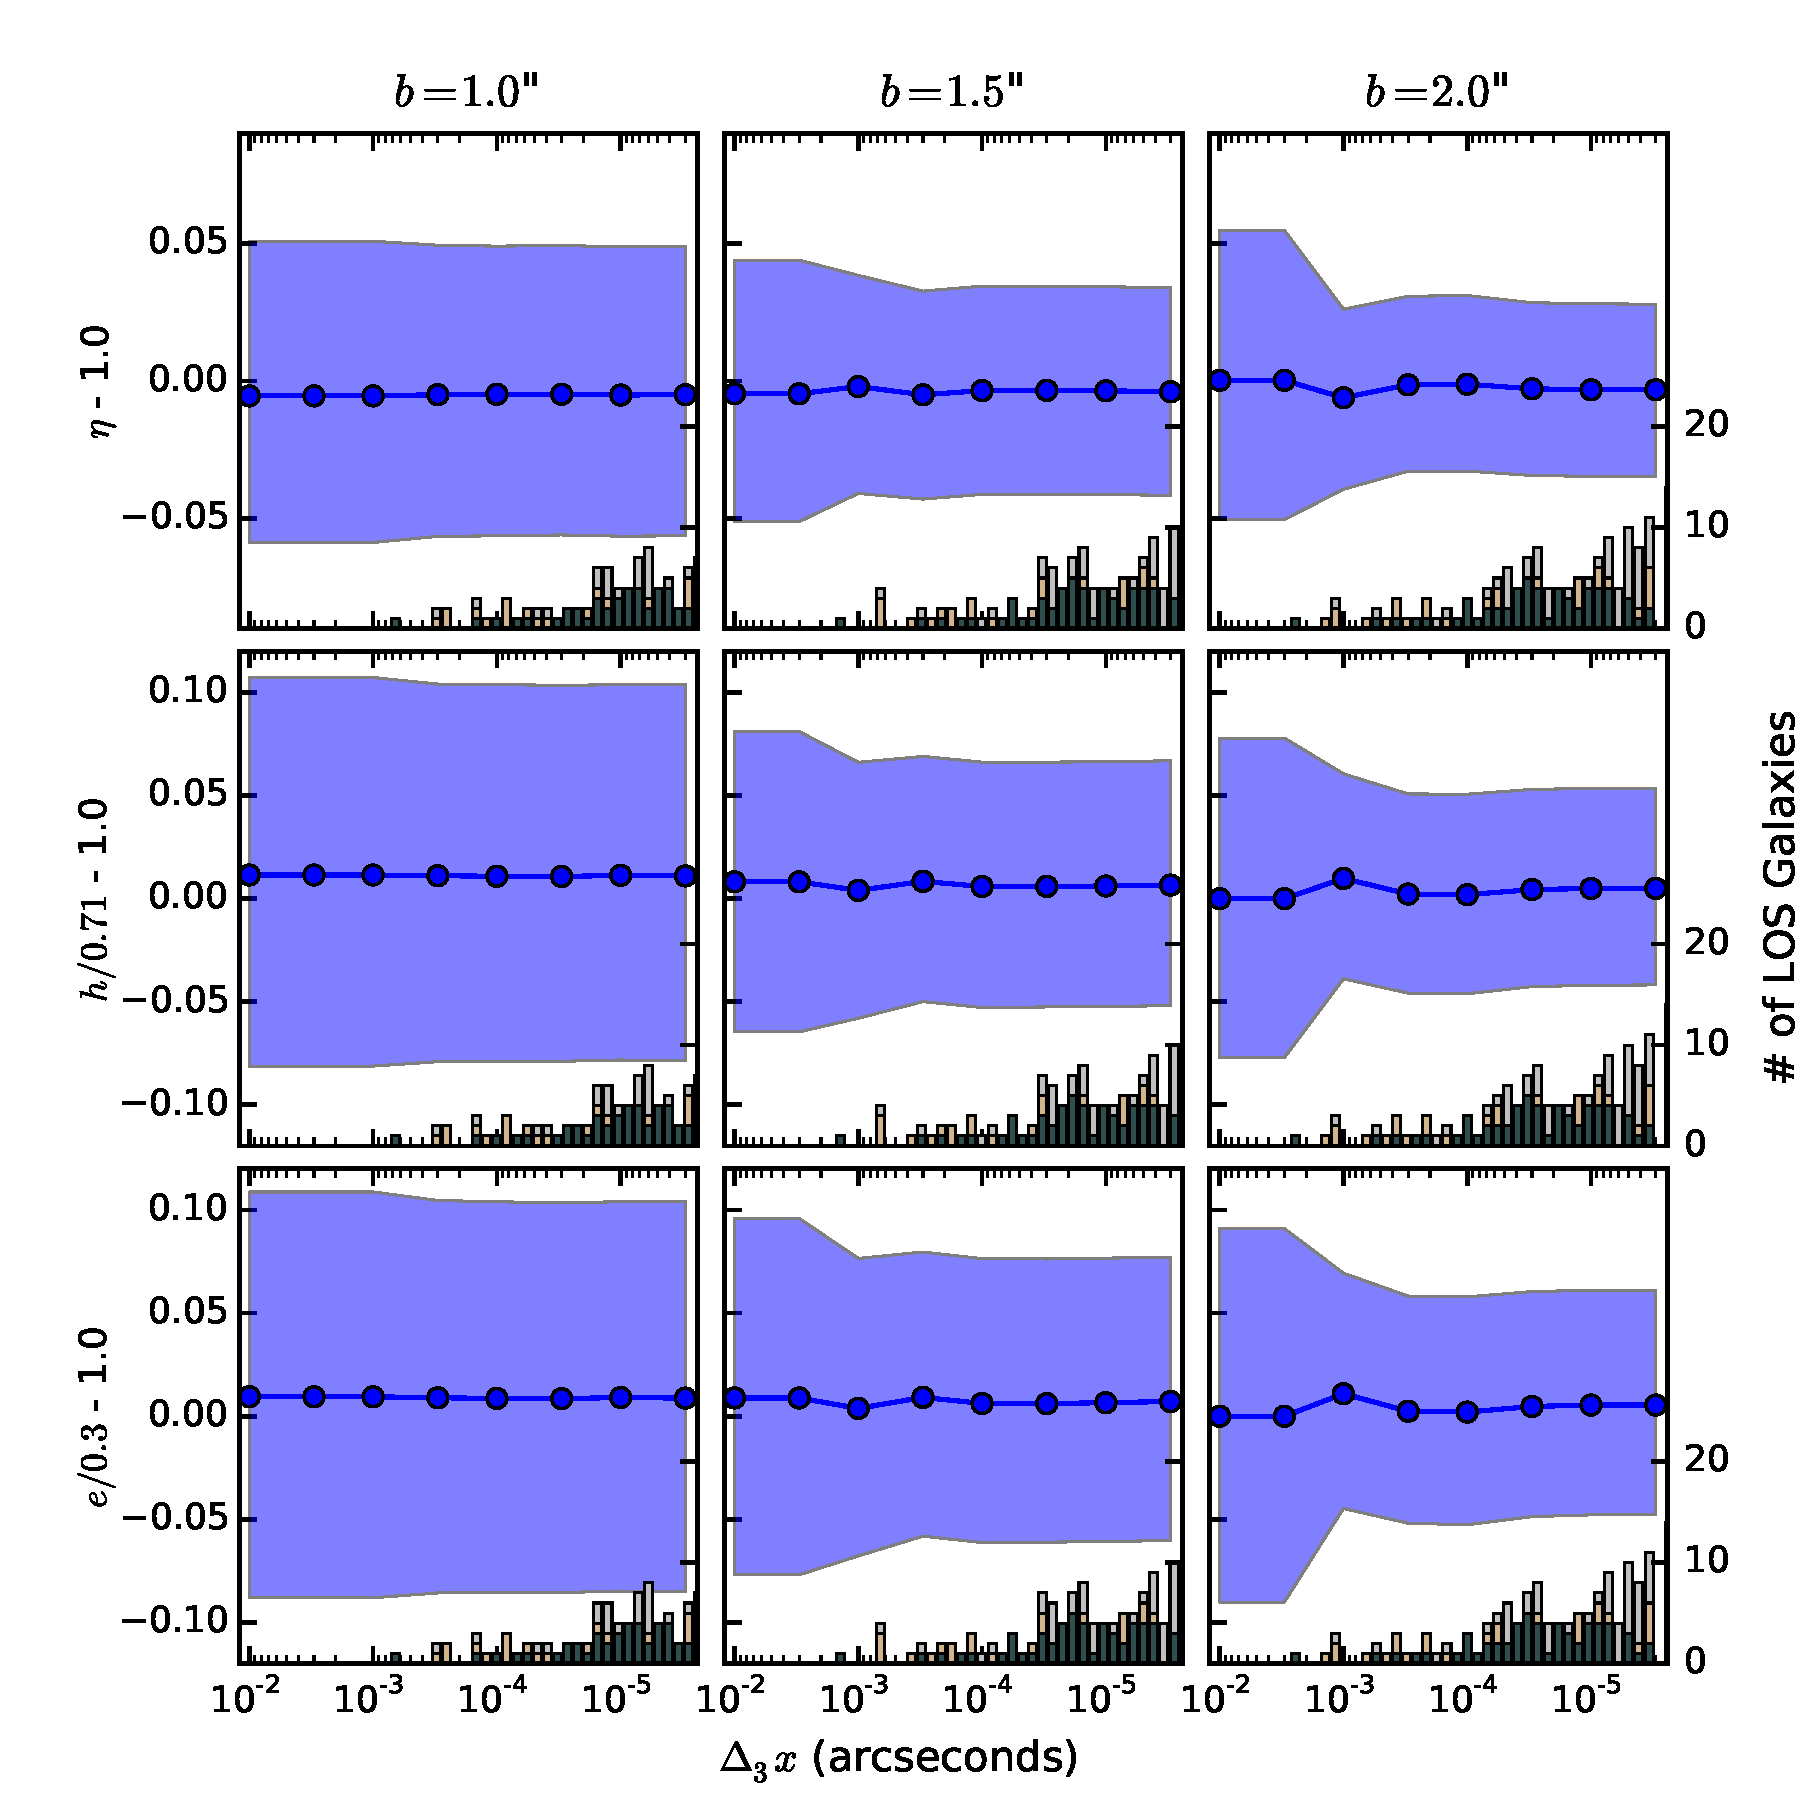
\includegraphics[width=1\textwidth]{recompare.pdf}
\caption{\label{fig:recompare} Similar to Figure \ref{fig:ecompare} but for different values of the Einstein radius parameter: $b = 1.0,1.5,2.0$ from left to right. Systems with a smaller Einstein radius have more scatter in the Hubble constant. Constraints on the ellipticity are somewhat stronger for lenses with larger Einstein radii, especially once the few strongest perturbers are included in models. This implies that lenses with a large Einstein radius should produce the strongest constraints on the Hubble constant.%
}
\end{center}
\end{figure*}

One possible approach to using gravitational lensing for precision cosmology is to search for one or a few ``golden lenses'' to use to measure cosmological parameters. One consideration when choosing these lenses needs to be the environment. The results in Figures \ref{fig:ecompare} and \ref{fig:recompare} show that asymmetric image configurations, e.g., those produced by a highly elliptical main lens galaxies, are less sensitive to the lens profile degeneracy leading to improved constraints on the Hubble constant.

The final system parameter we probe is the source position. In previous simulations, we have marginalized over the orientation of the main lens galaxy, which would wash out any trends we would see in the source plane. Instead, we now fix the lens system to match the real RXJ1131. \citet{Suyu13} find the best fit parameters of RXJ1131 to be $b = 1.64$'', $\eta = 1.05$, $e = 0.237$, and $\theta_e = 115.8^{\circ}$. We generate mock data for this configuration and then perform a modeling analysis as above, again treating all ENV/LOS galaxies in the tidal approximation.

Figure \ref{fig:srcpos} shows the median and scatter in the best fit Hubble constant as a function of source position. The models do well when the source is near a caustic. However, near the center of the caustic, both sets of models have larger scatter in the recovered values for the Hubble constant. These source positions correspond to more symmetric image configurations, with the exact center producing an Einstein ring. Symmetric image configurations produce weaker constraints on the ellipticity than asymmetric image configurations and are therefore more susceptible to lens profile degeneracy as discussed above.

\begin{figure}
\begin{center}
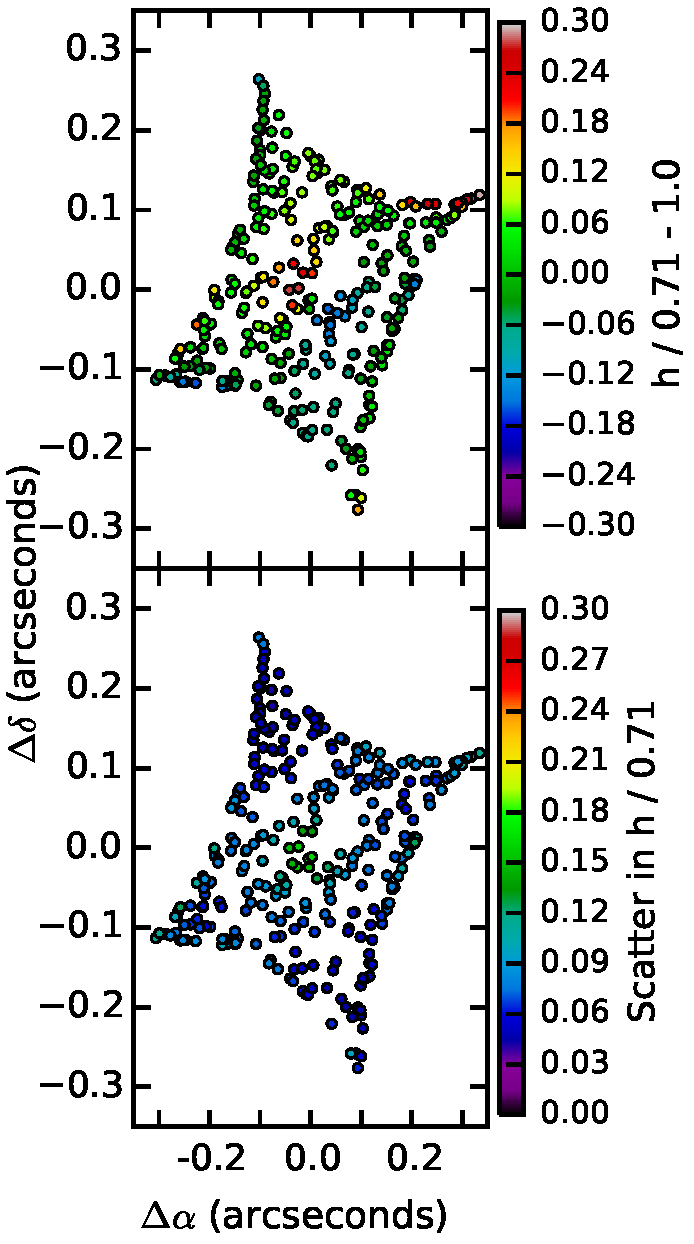
\includegraphics[width=1\columnwidth]{h_src_pos.pdf}
\caption{\label{fig:srcpos}
Median value (top) and scatter (bottom) for the recovered Hubble constant as a function of source position. The models have little bias and small scatter near caustics, but show an increased scatter/bias near the center. These central source positions correspond to more symmetric image configurations which produce weaker constraints on the ellipticity and are therefore more susceptible to the lens profile degeneracy. More asymmetric image configurations produce stronger contraints on the lens galaxy ellipticity and in turn on the Hubble constant.
}
\end{center}
\end{figure}

%%%%%%%%%%%%%%%%%%%%%%%%%%%%%%%%%%%%%%%%
\section{Conclusions}
%%%%%%%%%%%%%%%%%%%%%%%%%%%%%%%%%%%%%%%%

As lensing data improve, it becomes more important to take into account systematic effects like the perturbations due to galaxies in the environment and along the LOS. Our results show that if we want to do ``precision lensing,'' the environment and LOS cannot be ignored.

To understand and quantify how the ENV/LOS affects lensing, we have generated 3-D mass distributions based on photometric and spectroscopic observations. We then ray trace through these mass models to generate lensing observables. In these calculations, we self-consistently include the contribution from a smooth mass background, for the first time allowing us to account for mass (in)completeness and voids. We then fit the lensing observables with three types of models: Lens-Only models that ignore the environment, Lens+Shear models that take the common approach of fitting external shear as a free parameter, and our 3-D Lens models that treat ENV/LOS galaxies in the tidal approximation but include all non-linear effects from having mass at different redshifts.

We find that perturbers in the foreground of the lens affect the lens potential more than those in the background for two different reasons. The first is that background perturbers are downweighted; a background perturber must be closer in projection to have the same effect as a foreground perturber. The second is that while background perturbers can be mimicked by a shear in the lens plane, foreground perturbers create non-linear effects that cannot be fit with a simple external shear.

Using our results based on individual perturbing galaxies, we define a quantity that we have termed the ``flexion shift'', $\Delta_3 x$ (eqs.\ \ref{eqn:backgroundd3x} and \ref{eqn:foregroundd3x}), to characterize the ENV/LOS contributions to the lens potential.

Using this quantity, we find that the importance of environment/LOS effects varies significantly from field to field. Therefore, we argue that each field needs to be modeled individually. Even accounting for the uncertainties in building the 3-D mass models, we find that directly calculating the external converenge from the 3-D mass models produces a narrower distribution than that from ray tracing through N-body simulations. This translates to a stronger prior on measuring the Hubble constant. We find that lens galaxies that are in groups tend to have a stronger contribution from the ENV/LOS than those that are not in groups. 

We show that fitting lens models that ignore the ENV/LOS does not reproduce the input lens system parameters or the Hubble constant. Models that fit an external shear, the Lens+Shear models, overpredict the Hubble constant and the Einstein radius of the main lens galaxy; these quantities need to be corrected using some other constraint on the external convergence, typically done in post processing. Our 3-D lens models do not produce this bias because we explicitly include the convergence in the lens models.

We show that all models, including both the Lens+Shear and 3-D Lens models, are subject to the lens profile degeneracy in agreement with \citet{Xu15,Schneider13}. Extra information like kinematic measurements or extended source reconstruction techniques are necessary.

For either methodology of fitting an external shear or using our LOS framework, we still must choose which galaxies are treated exactly and which are treated in the tidal approximation. We find that we can reproduce the true lens parameters with no bias and a scatter less than the observational uncertainties if we use a cutoff in $\Delta_3 x$ of $10^{-4}$ arcseconds, a factor of 30 smaller than the assumed uncertainties on the observed positions. This cut typically requires 10-15 galaxies of $\sim 300$ galaxies within 5 arcminutes to be treated exactly, making the calculation $\sim 400-900$ times more efficient than the full multi-plane lens equation.

LSST will find an immense number of new strong lens systems. There are various strategies about how to use this upcoming dataset for cosmology. One possibility is to use all of the lenses to beat down uncertainties using statistics. However, if we are entering the systematics-limited regime, this approach will succeed only if one can account for systematic uncertainties (e.g., with our 3-D Lens models). An alternative strategy is to use the large number of lenses discovered by LSST to search for a few rare, ``golden'' lenses that have small systematic uncertainties. One possible criterion for a ``golden'' lens could be to have a weaker contribution from the environment/LOS. Based on our analysis, to minimize environment/LOS effects, we should search for lenses with a large Einstein radius and high ellipticity. These large, asymmetric lenses will be less sensitive to the lens profile degeneracy. While suggestive, these results merit further investigation to get the most out of future surveys like LSST.

Throughout this work we have assumed that our 3-D models perfectly describe the environment/LOS, but there is also uncertainty in generating the environment mass models that is only briefly addressed here. This source of uncertainty will be explored in a forthcoming paper (Wong et al., in prep.).

\acknowledgements
We thank Phil Marshall, Sherry Suyu, Chris Fassnacht, and Stefan Hilbert for enlightening discussions about 3-D lensing. CVM acknowledges support from NSF grant AST-1313484. CRK acknowledges funding from NSF grant AST-1211385. AIZ acknowledges funding from NSF grant AST-1211874 and NASA grant ADP-10AE88G. She also thanks the John Simon Guggenheim Foundation and the Center for Cosmology and Particle Physics at NYU for their support. KCW is supported by an EACOA Fellowship awarded by the East Asia Core Observatories Association, which consists of the Academia Sinica Institute of Astronomy and Astrophysics, the National Astronomical Observatory of Japan, the National Astronomical Observatories of the Chinese Academy of Sciences, and the Korea Astronomy and Space Science Institute.


\bibliographystyle{apj}
\bibliography{sims}

\end{document}